%%%%%%%%%%%%%%%%%%%%%%%
% Theoretical Background
%%%%%%%%%%%%%%%%%%%%%%%%

\chapter{Introduction}\label{chap:1}

\section{Overview}\label{sec:bkgrd_overview}
Fluid motions driven by buoyancy and frictional forces belongs to class of flows known as thermoconvective shear flows.
These flows exhibit rich behaviour, and are of interest in both engineering and meteorology applications spanning across a broad range of length scales.

\begin{figure}[ht]
    \centering
    \begin{tikzpicture}[scale=1.3]
        \node at (0,0) {\includegraphics[width=0.2\textwidth]{Background/Figures/Applications/chipcooling.jpg}};
        \node at (0,1.5) {(a) Chip cooling};
        \node at (3.5,0) {\includegraphics[width=0.3\textwidth]{Background/Figures/Applications/CVD.png}};
        \node at (3.5,1) {};
        \node [label={[align=center] (b) Chemical Vapor\\Deposition}] at (3.5,0.7) {};
        \node at (7.8,1.3) {\includegraphics[width=0.3\textwidth]{Background/Figures/Applications/cloudstreets.jpg}};
        \node [label={[align=center] (c) Cloud Streets}] at (7.9, 3.8) {};
        \draw [-, black] (0.1,-1.6) -- (0.1,-1.4);
        \node at (0.1,-1.8) {$10^{-2}$};
        \draw [-, black] (3.5,-1.6) -- (3.5,-1.4);
        \node at (3.5,-1.8) {$10^1$};

        \draw [-, black] (7.5,-1.6) -- (7.5,-1.4);
        \node at (7.5,-1.8) {$10^3$};

        \node [label={[align=center] $L$ $(m)$}] at (9.8,-2.2) {};
        \draw [->, thick, black] (-1,-1.5) -- (10,-1.5);
        % \draw [->, thick, white] (0,-1.8) -- (8.1,-1.8);
    \end{tikzpicture}
    \label{fig:applications}
    \caption{Thermoconvective shear flows driven by shear and bouuyancy forces across length scales, $L \in [10^{-2}m, 10{^3}m]$. Examples include (a) chip cooling, (b) chemical vapour deposition and (c) the formation of cloud streets.}
\end{figure}


At small scales, around $L \sim 10^{-2} m$ \textcolor{red}{(figure \ref{fig:applications}(a))}, thermoconvective flows are relevant to the cooling of microprocessing chips.
The fluid, acting as a medium for dissipating heat \textcolor{red}{generated by the chips}, experiences shear and buoyancy forces from the \textcolor{red}{confine walls, and heat.}
One of the major challenge in this industry is on increasing the density of transistors on a single chip.
\textcolor{red}{Moore's Law predicts} the doubling of transistors on a single chip approximately every two years.
One of the major limitations is the challenge of dissipating the excessive heat generated from the densely packed transistors.
Fluids, such as air, water or refrigerants, are often used to transport heat away from the components, and their transport behaviour under the influence of buoyancy and shear remains an open topic \citep{kennedy_combined_1983, ray_analysis_1992}.

At intermediate length scales, $L \sim 1m$ \textcolor{red}{(figure \ref{fig:applications}(b))}, the interaction between buoyancy and frictional forces is important in the fabrication of uniform thin films in chemical vapour deposition (CVD) \citep{evans_unsteady_1991,jensen_flow_1991}.
\textcolor{red}{The CVD process consist of transporting reactive gaces flowing over a heated substrate.}
% The CVD process typically involves a reactive gases carried by inert gases which flows through a channel with a heated substrate.
Upon heating, the reactant gases react chemically on the substrate, depositing material and forming thin films, such as silicon layers.
A key challenge in the CVD process is achieving a uniform deposition and maintaining sharp interfaces between layers.
The interactions between shear and buoyancy forces often gives rise to boundary layers and thermoconvective rolls, which can disrupt uniform deposition, affecting fillm quality.

At larger length scales, $L \sim 10^3m$, the thermoconvective shear flows can be observed in atmospheric flows such as the cloud streets over the Norwegian Sea. 
These parallel bands of cumulus clouds can stretch over hundreds of kilometres.
They form when the relatively warmer sea surface heat up the colder air arriving from the North pole.
As the colder air is heated, it rises upwards whilst carrying water vapour, condensing into visible clouds.
This ciruclation is organised into parallel rotating parallel columns of air, forming distinct cloud streets.

The central focus of this thesis is on the investigation of fluid behaviour arising from the interaction between shear and buoyancy forces, \textcolor{red}{common among} the physical examples discussed above.
We note that by isolating our analysis to the interaction between shear and buoyancy forces, we might neglect other physical mechanisms such as phase change, chemical reactions and evaporation, which may be significant in the context of cooling microproccessors, chemical vapour deposition, and atmopsheric boundary layers respectively \citep{vallis_simple_2019}.
Nonetheless, the interaction between shear and buoyancy forces remains an open topic and will be the primary focus of this thesis, providing a foundation for future investigations that may include addition mechanisms.


To consider this interaction, we consider an idealised setup, known as the Rayleigh-B\'{e}nard-Poiseuille (RBP) flow.
This RBP system describes the fluid motion confined between two infinitely extended parallel \textcolor{red}{walls}, heated from below and cooled from the top, with an additional pressure gradient driving the flow.
The RBP configuration combines the two paradigmatic flow configurations; the classical Rayleigh-B\'{e}nard convection (RBC) and plane Poiseuille flow (PPF), driven by buoyancy and shear, respectively.
While the onset of convection in RBC, and the transition to subscritical shear-driven turbulence in PPF have been both extensively studied, the transitional regime in which both forces interact remains less understood.
Understanding their transitional behaviour and transport properties could have direct implications for the physical examples mentioned above.

\begin{figure}[h]
\centering
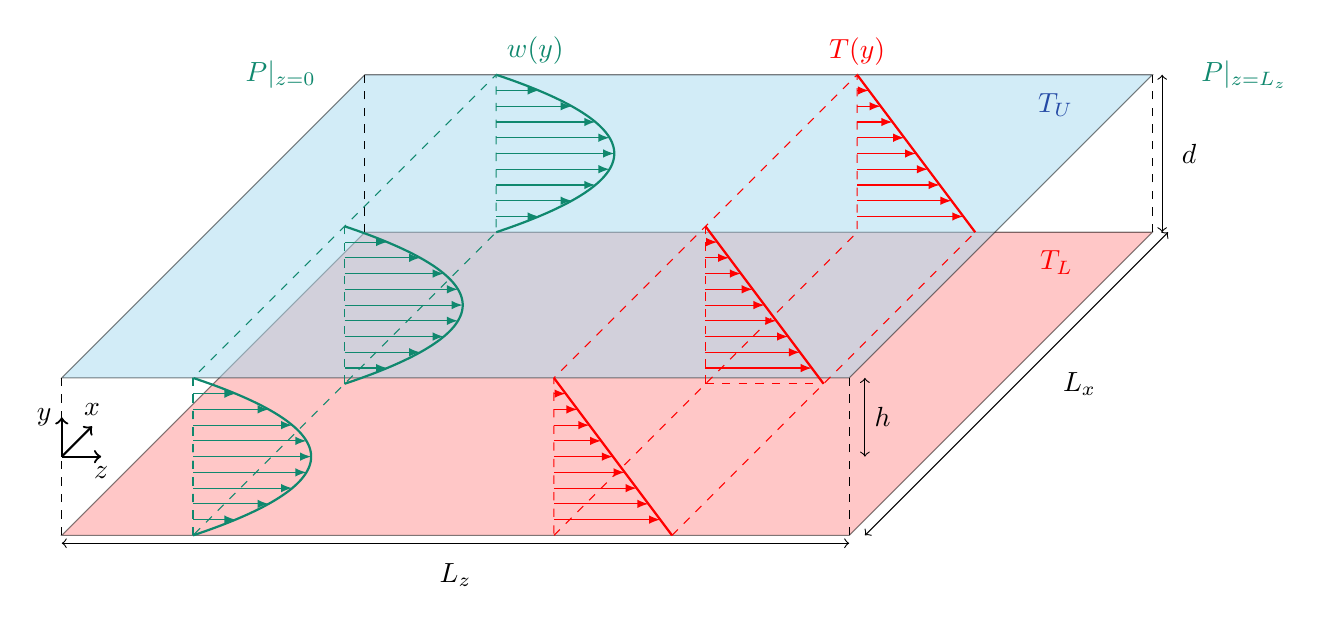
\begin{tikzpicture}
\def\H{1}
\def\W{10}
\def\L{10}

% Draw the bottom plate
\draw [fill=pink!75!red, opacity=0.5] (-\L/2,-\H,0) -- (\L/2,-\H,0) -- (\L/2, -\H, -\W) -- (-\L/2, -\H,-\W) -- cycle;

% Draw the top plate
\draw [fill=SkyBlue!75!white, opacity=0.5] (-\L/2,\H,0) -- (\L/2,\H,0) -- (\L/2, \H, -\W) -- (-\L/2,\H,-\W) -- cycle;

%  % Draw axes
\draw [dashed, thin] (-\L/2, -\H, 0) -- (-\L/2, \H, 0);
\draw [dashed, thin] (\L/2, -\H, 0) -- (\L/2, \H, 0);
\draw [dashed, thin] (\L/2, -\H, -\W) -- (\L/2, \H, -\W);
\draw [dashed, thin] (-\L/2, -\H, -\W) -- (-\L/2, \H, -\W);
%\draw [dashed, thin] (-1,0, 0) --++ (\L,0,0) --++ (0,0,-\W) --++ (-\L,0,0) -- cycle;
%  % \draw [thin, dashed] (-1,0) -- (6,0);

% Add dimensions
% L_x
\draw [<->] (-\L/2,-1.1*\H, 0) -- (\L/2,-1.1*\H,0);
\node[centered] at (0,-1.5*\H,0) {$L_z$};
 
% L_z
\draw [<->] (\L/2*1.025, -\H, -\W) -- (\L/2*1.025, \H,-\W);
\node[right] at (\L/2*1.05,0.0,-\W) {$d$};

% d
\draw [<->] (\L/2*1.04, -\H) -- (\L/2*1.04,-\H,-\W);
\node[centered] at (\L/2*1.2,-\H,-\W/2) {$L_x$};

% h
\draw [<->] (\L/2*1.04, 0, 0) -- (\L/2*1.04, \H, 0);
\node[right] at (\L/2*1.04,\H/2,0) {$h$};

% P
\node[left] at (-\L/2*1.1, \H, -\W) {\textcolor{PineGreen}{$P|_{z=0}$}};
\node[right] at (\L/2*1.1, \H, -\W) {\textcolor{PineGreen}{$P|_{z=L_z}$}};

% T
\node[left] at (\L/2*0.9, \H, -\W*0.9) {\textcolor{cyan!20!blue}{$T_U$}};
\node[left] at (\L/2*0.9, -\H, -\W*0.9) {\textcolor{red}{$T_L$}};

% Draw labels
\draw[->, thick] (-\L/2, 0, 0) -- (-\L/2,\H/2,0) node[left] {$y$};
\draw[->, thick] (-\L/2, 0, 0) -- (-\L/2+\H/2,0,0) node [below] {$z$};
\draw[->, thick] (-\L/2, 0, 0) -- (-\L/2,0,-\H) node[above] {$x$};

% Draw the velocity profile
\draw[PineGreen,thick,domain=-1:1,samples=200,smooth] plot ({(1-\x*\x)*1.5-\L/3}, \x) node[above right] {};
\draw[PineGreen,thick,domain=-1:1,samples=200,smooth] plot ({(1-\x*\x)*1.5-\L/3}, \x, -\W/2) node[above right] {};
\draw[PineGreen,thick,domain=-1:1,samples=200,smooth] plot ({(1-\x*\x)*1.5-\L/3}, \x, -\W) node[above right] {$w(y)$};
\draw[-,PineGreen,dashed] (-\L/3,-\H) -- (-\L/3,\H);
\draw[-,PineGreen,dashed] (-\L/3,-\H, -\W/2) -- (-\L/3,\H, -\W/2);
\draw[-,PineGreen,dashed] (-\L/3,-\H,0) -- (-\L/3,\H,0) -- (-\L/3,\H,-\W) -- (-\L/3,-\H,-\W) -- cycle;

\foreach \y in {-0.8,-0.6,...,0.8} {
    \draw[-latex,PineGreen] (-\L/3,\y, 0) -- ({(1-\y*\y)*1.5-\L/3},\y,0);
    \draw[-latex,PineGreen] (-\L/3,\y, -\W/2) -- ({(1-\y*\y)*1.5-\L/3},\y, -\W/2);
    \draw[-latex,PineGreen] (-\L/3,\y, -\W) -- ({(1-\y*\y)*1.5-\L/3},\y,-\W);
}

% Draw the temperature profile
\draw[red,thick,domain=-\H:\H,samples=200,smooth] plot ({(1/2*(1-\x)*1.5+\L/8)}, \x);
\draw[red,thick,domain=-\H:\H,samples=200,smooth] plot ({(1/2*(1-\x)*1.5+\L/8)}, \x, -\W/2);
\draw[red,thick,domain=-\H:\H,samples=200,smooth] plot ({(1/2*(1-\x)*1.5+\L/8)}, \x, -\W);
\draw[-,red,dashed] (\L/8,-\H,-\W/2) -- (\L/8,\H,-\W/2);
\draw[-,red,dashed] (\L/8,-\H,-\W/2) -- (\L/8 + 1.5,-\H,-\W/2);
\draw[-,red,dashed] (\L/8 +1.5,-\H,0) -- (\L/8 + 1.5,-\H,-\W);
\draw[-,red,dashed] (\L/8,-\H,0) -- (\L/8,-\H,-\W) -- (\L/8,\H, -\W) -- (\L/8,\H,0) -- cycle;
% % 
\foreach \y in {-0.8,-0.6,...,0.8} {
   \draw[-latex,red] (\L/8,\y) -- ({\L/8+(1/2*(1-\y)*1.5},\y);
   \draw[-latex,red] (\L/8,\y, -\W/2) -- ({\L/8+(1/2*(1-\y)*1.5},\y, -\W/2);
   \draw[-latex,red] (\L/8,\y, -\W) -- ({\L/8+(1/2*(1-\y)*1.5},\y, -\W);
}
% Add labels
\node[above,red] at (\L/8,1,-\W) {$T(y)$};
\end{tikzpicture}
\label{fig:rbpconfiguration}
\caption{The Rayleigh-B\'{e}nard Poiseuille (RBP) flow configuration.}
\end{figure}


The RBP configuration is illustrated in figure \ref{fig:rbpconfiguration}, where $z,y,x$ refer to spatial coordinates denoting the streamwise, spanwise and wall normal directions.
$L_z, L_x, d$ and $h$ corresponds to the length, span, depth and half-height of the domain respectively.
The RBP system is biperiodic along $z$ and $x$.
% We note that the asterisks$^*$, refer to variables in dimensional form.
The flow is driven by a pressure gradient along the streamwise $z$ direction, $\Delta P = P|_{z=0} - P|_{z=L_z} < 0$, leading to a laminar Poiseuille flow, $w(y) = W_c(1 - y^2)$, where $W_c$ is the laminar centerline velocity.
We consider a fully developed flow, where the boundary layer developing from the top and the bottom wall meets at the midplane $y=0$ and entrance effects are therefore neglected.
Like the RBC system, the RBP system is unstably stratified \textcolor{red}{due to temperature differences}.
The temperature difference between the lower, $T_L$, and upper wall, $T_U$, is always positive, $\Delta T = T_L - T_U > 0$, leading to a stable linear conduction layer along the wall-normal direction, $T(y)$, if $\Delta T$ is kept sufficiently small.
The behaviour of RBP flows is govern by four dimensionless parameters,
\begin{equation}\label{eq:nondim_def}
    Re = W_c h / \nu, \quad Ra = \frac{\eta g d^3 \Delta T}{\nu \kappa}, \quad Pr = \frac{\kappa}{\nu}, \quad \Gamma = L/2d,
\end{equation}
where $Ra, Re, Pr, \Gamma$ refers to Reynolds, Rayleigh, Prandtl numbers and aspect ratio and 
$\eta, g, \nu, \kappa,$ are the thermal expansion coefficient, acceleration due to gravity, kinematic viscosity, thermal diffusivity, respectively.
The Reynolds number, $Re$, and the Rayleigh number, $Ra$, are dimensionless parameters that characterise the relative influence of shear and buoyancy respectively.
For sufficiently large values of $Re$ and $Ra$, RBP flows may undergo a transition to shear-driven turbulence or convection-driven convection.
In the absence of shear, $Re = 0$, the RBP configuration reduces to the classical buoyancy driven Rayleigh-B\'{e}nard convection, which forms a bistable system between stationary and chaotic convection rolls slightly above the \textcolor{red}{critical $Ra$ (see \S \ref{sec:bkgrd_RBC}).}
The influence of $Re$ on \textcolor{red}{the behaviour of the bistable system} remains unexplored.

In the first part of this thesis, we focus on the transitional regime by investigating whether buoyancy forces promote the transition to shear-driven turbulence and examing the effect of shear on convection in large domains. 
The second part of this thesis explore the state space structure of a bistable system between a chaotic convection roll state and a stationary convection roll state of Rayleigh-B\'{e}nard convection.
% In the limiting case without unstable stratification, $Ra = 0$, the system reduces to the wall-bounded plane Poiseuille flow (PPF), where the transition towards subscritical shear-driven turbulence may be expected for a sufficiently large pressure gradient.
% For instance, do buoyancy forces promote the transition to shear-driven turbulence and how does shear influence the convection? 
% To describe the motion of the fluid in RBP configurations, we consider the non-dimensionalised Navier-Stokes equations with Boussinessq approximations,
% \begin{subequations}\label{eq:rbp_equations}
% \begin{equation}
%     \frac{\partial \mathbf{u}}{\partial t} + (\mathbf{u}\cdot\nabla)\mathbf{u} = -\nabla p + \frac{1}{Re}\nabla^2 \mathbf{u} + \frac{Ra}{Re^2Pr} \theta,
% \end{equation}
% \begin{equation}
%     \frac{\partial \theta}{\partial t} + (\mathbf{u} \cdot \nabla)\theta = \frac{1}{RePr}\nabla^2 \theta,
% \end{equation}
% \begin{equation}
%     \nabla \cdot \mathbf{u} = 0.
% \end{equation}
% \end{subequations}
% where $\mathbf{u}(\mathbf{x}), \theta(\mathbf{x}), p(\mathbf{x})$ refers to the nondimensionalised velocity, temperature and presure respectively.
% The key control parameters for RBP flows are the Rayleigh number, $Ra$, Reynolds number, $Re$, Prandlt number $Pr$, which are defined as follows,
% \begin{equation}
%     Ra = \eta g d^3 \Delta T / \nu \kappa, \quad Re = W_c h / \nu, \quad Pr = \kappa / \nu, \quad \Gamma = L/2d,
% \end{equation}
% where $\eta, g, \Delta T, \nu, \kappa, W_c, h, d, L$ are the thermal expansion coefficient, acceleration due to gravity, temperature difference between the bottom and top wall, kinematic viscosity, thermal diffusivity, laminar centreline velocity, domain's half-depth, full-depth, length or span respectively.

The structure of this introductory chapter is as follows:
we begin our discussion on the development of hydrodynamic stability theory of wall-bounded shear flows in \S \ref{sec:bkgrd_transitional}.
Theoretical frameworks used in the study of the stability of fluid flow, including linear modal/non-modal stability, nonlinear dynamical systems and the spatio-temporal dynamics of transitional shear flows will be discussed.
Throughout \S \ref{sec:bkgrd_transitional}, we apply these concepts in the context of plane Poiseuille flows (PPF).
\textcolor{red}{The developments of Rayleigh-B\'{e}nard convection (RBC) is followed in \S \ref{sec:bkgrd_RBC}.}
Finally, we review the developments in RBP flows \S \ref{sec:bkgrd_RBP}, before concluding this chapter with an outline of the thesis in \S \ref{sec:bkgrd_thesis_outline}.


% We first discuss the key developments of plane Poiseuille flow (PPF) outlining the key theoretical framework for analysing the stability of fluid flows. This is then followed by Rayleigh-B\'{e}nard convection (RBC) in \S \ref{sec:bkgrd_RBC}.

%%%%%%%%%%%%%%%%%%%%%%%%
% Plane Poiseuille Flows
%%%%%%%%%%%%%%%%%%%%%%%%

\section{Transitional wall-bounded shear flows}\label{sec:bkgrd_transitional}
Wall-bounded shear flows concerns the motion of the fluid flowing in parallel to walls, typically bounded by one or more walls.
Near the wall, the fluid comes to rest due to the no-slip boundary condition, resulting in a velocity gradient perpendicular to the wall, giving rise to shear within the fluid, \textcolor{red}{defining \textit{wall-bounded shear flows}.}
% The fluid closest to the wall comes to a rest, satisfying the no-slip boundary condition in the presence of a wall.
% As a consequence, a velocity gradient in the direction perpendicular from the wall develops, where the fluid layer becomes \emph{sheared} due to the pressence of the wall - referred to wall-bounded sheared flows.
% In Newtonian fluids, shear stresses are directly proportionate to the velocity gradient by the fluids kinetic viscosity, $\nu$, given as,
% \begin{equation}\label{eq:shear}
%    \tau = \nu \frac{\partial u}{\partial y},
% \end{equation}
% where $\tau$, $\nu$, and $\frac{\partial u}{\partial y}$ refers to shear stresses - hence wall-bounded shear flows.
Examples include the pressure-driven plane Poiseuille flow (channel flow), Hagen-Poiseuille flow (pipe flow), plane Couette flow and flat plate boundary layers.
These geometrically simple configurations provides a convenient framework amenable to the mathematical analysis of fluid motion subjected to shear.
Depending on the degree of shear, the fluid motion can be either laminar, where the fluid layers move in smooth parallel 'laminates', or turbulent, characterised by chaotic eddying motions.
We also note that there is a transitional regime where both states can coexist discuss later.
A central question is predicting the transition from the laminar regime to the turbulence.
% One of the central questions is on the prediction on the transition to turbulence, specifically, when is turbulence expected as shear is increased?
% plane Poiseuille flow (PPF) describes the motion of a fluid confined between two infinitely extended parallel walls, driven by a pressure gradient, also referred to as channel flow.
% It belongs to a general class of wall-bounded shear flows, consisting of plane Couette flow, pipe (Hagen-Poiseuille) flow and flat plate boundary layer flow.

The first \textcolor{red}{systematic} investigation into this transition was conducted by \cite{reynolds_xxix_1883}.
% The earliest investigation into this transition dates back to the pipe flow experiments of \cite{reynolds_xxix_1883}.
In his experimental setup, the flow speed through the pipe could be controlled by regulating the inlet pressure, while injecting dye to visualise the flow, as illustrated in figure \ref{fig:reynolds}(a).
At low speeds, the fluid remained laminar, resulting to a single streak of steady dye in figure \ref{fig:reynolds}(b).
As the speed increased, the dye begin to exhibit irregular `sinuous' motions interspersed with laminar regions shown in figure \ref{fig:reynolds}(c).
This is now referred to as the transitional regime, alternating between the laminar and turbulent states.
Beyond a critical speed, the dye breaks down entirely into chaotic `eddies', mixing with the surrounding fluid and discolouring the flow with dye downstream in figure \ref{fig:reynolds}(d).
This regime is now identified as turbulence.

Reynolds proposed that the threshold between the laminar, transitional and turbulent regimes could be characterised by a non-dimensional parameter, now referred to as the Reynolds number,
\begin{equation}
    Re = U D/\nu,
\end{equation}
where $U$ is the centerline velocity in the pipe, $D$, the pipe diameter and $\nu$, the kinematic viscosity.
He observed that flow through the pipe remained \textit{stable} and laminar for $Re < 1900$, while it became \textit{unstable} and turbulent for $Re > 2000$ \citep{reynolds_iv_1895}, introducing the notion of flow \textit{stability}.
\begin{figure}[h]
    \centering
    \includegraphics[width=1\textwidth]{Background/Figures/Reynolds.pdf}
    \caption{(a) Osbourne Reynolds pipe experiment with the dye injection apparatus, illustrating the (b) laminar flow, (c) transitional regime and (d) turbulent flow as the flow speed is increased, taken from \protect\cite{reynolds_xxix_1883}.}
    \label{fig:reynolds}
\end{figure}

%%%%%%%%%%%%%%%%%%%%%%%%%%%
% Linear Stability Analysis
%%%%%%%%%%%%%%%%%%%%%%%%%%%

\subsection{Linear Stability Analysis}
Following Reynolds' experiment, interest towards the mathematical analysis of the stability of laminar flows grew in early $20^{st}$ century.
The mathematical approach typically begins by decomposing the velocity field, $\mathbf{u}(\mathbf{x},t)$, into a laminar (base) state, $U(y)$, and the velocity perturbations, $\mathbf{u}'(\mathbf{x},t)$, with pressure similarly decomposed as,
\begin{equation}
    \mathbf{u}(\mathbf{x}) = U(y) + \mathbf{u}'(\mathbf{x},t), \quad \text{and} \quad p(\mathbf{x},t) = P(x) + p'(\mathbf{x},t).
\end{equation}
Substituting into the Navier-Stokes equations and linearising (neglecting nonlinear terms), we get,
% Next, we the substitute the formulations for the decomposed velocity and pressure into the Navier-Stokes equations of equation \eqref{eq:rbp_equations} and drop the nonlinear pertubrations terms $(\mathbf{u'}\cdot \nabla)\mathbf{u'}$,
\begin{subequations}\label{eq:shear_linearised}
\begin{equation}
    \frac{\partial \mathbf{u'}}{\partial t} + (U \cdot\nabla)\mathbf{u'} + (\mathbf{u'}\cdot\nabla)U= -\nabla p' + \frac{1}{Re}\nabla^2 \mathbf{u'},
\end{equation}
\begin{equation}
    \nabla \cdot \mathbf{u}' = 0,
\end{equation}
\end{subequations}
known as the linearised Navier-Stokes equations. 
This commonly followed by introducing a wavelike ansatz (mode) for the perturbations, and analysed by considering their behaviour independently, referred to as modal analysis in \S \ref{subsec:modal}, or their coupled dynamics, referred to as non-modal analysis in \S \ref{subsec:nonmodal}.

% In general two ways to analysis the linearised Navier-Stokes equations by considering the behaviour of each mode independently in \S \ref{subsec:modal} and their coupled dynamics in \S \ref{subsec:nonmodal}

%%%%%%%%%%%%%%%%%
% MODAL STABILITy
%%%%%%%%%%%%%%%%%

\subsubsection{Modal analysis}\label{subsec:modal}
It is covenient to eliminate the pressure terms by reformulating equation \eqref{eq:shear_linearised} using the wall-normal perturbation velocity, $v'$, and wall-normal vorticity, $\eta' = \partial u'/ \partial z - \partial w' / \partial x$, variables.
Using $(v, \eta)$, we introduce a modal ansatz for them,
\begin{equation}\label{eq:shear_ansatz}
    v'(\mathbf{x},t ) = \tilde{v}(y)e^{i(\alpha x + \beta z - \omega t)}, \quad \text{and} \quad \eta'(\mathbf{x}, t) = \tilde{\eta}(y)e^{i(\alpha x + \beta z - \omega t)}.
\end{equation}
where $\alpha, \beta, \omega$ denotes the streamwise and spanwise wavenumbers, and complex frequency (i.e. $\omega = \omega_r + i\omega_i$), respectively.
Substituting this ansatz into \textcolor{red}{the} linearised equations \textcolor{red}{leads} to the classical Orr-Sommerfeld and Squire equations \citep{orr_stability_1907,sommerfeld_beitrag_1909,squire_stability_1933, schmid_stability_2001},
% \begin{equation}
%     \mathbf{L}\mathbf{\tilde{q}} = i\omega\mathbf{M}\mathbf{\tilde{q}}
% \end{equation}
\begin{subequations}
\begin{equation}\label{eq:OSQ}
    \begin{pmatrix}
        \mathcal{L}_{OS} & 0 \\
        i\beta U' & \mathcal{L}_{SQ}
    \end{pmatrix}
    \begin{pmatrix}
        \tilde{v} \\
        \tilde{\eta}
    \end{pmatrix}
    = 
    i\omega
    \begin{pmatrix}
        k^2 - \mathcal{D}^2 & 0 \\
        0 & 1 
    \end{pmatrix}
    \begin{pmatrix}
        \tilde{v} \\
        \tilde{\eta}
    \end{pmatrix}.
\end{equation}
% \begin{equation}\label{eq:OSQ}
%     \left[
%     -i\omega 
%     \begin{pmatrix}
%         k^2 - \mathcal{D}^2 & 0 \\
%         0 & 1 
%     \end{pmatrix}
%     + 
%     \begin{pmatrix}
%         \mathcal{L}_{OS} & 0 \\
%         i\beta U' & \mathcal{L}_{SQ} 
%     \end{pmatrix}
% \right ]
%     \begin{pmatrix}
%         \tilde{v} \\
%         \tilde{\eta}
%     \end{pmatrix}
%     = \mathbf{0},
% \end{equation}
\text{with}
  \begin{equation} 
      \mathcal{L}_{OS} = i\alpha U(k^2-\mathcal{D}^2) + i\alpha U'' + \frac{1}{Re}(k^2 - \mathcal{D}^2)^2,
      \quad \mathcal{L}_{SQ} = i\alpha U + \frac{1}{Re}(k^2 - \mathcal{D}^2).
  \end{equation}
\end{subequations}
where $\mathcal{D} = d/dy, k^2 = \alpha^2 + \beta^2$ and $U''$ is the second derivative of $U(y)$.
% $k^2, \mathcal{D}, U', U''$ denotes the sum of squared wavenumbers, $k^2 = \alpha^2 + \beta^2$, differential operator in $y$, first- and second- derivative of the laminar velocity, respectively.
Equation \eqref{eq:OSQ} is an generalised eigenvalue problem with eigenvalue $i\omega$, which determines the growth of perturbations.

The goal of modal stability analysis is to determine the critical Reynolds number $Re_c$, defined as the lowest value of $Re$, for all $\alpha$ and $\beta$ in which $\Im[\omega] = 0$.
For $Re > Re_c$, perturbations can grow exponentially, indicating instability.
% For $Re > Re_c$, perturbations could grow exponentially, departing from the laminar state.
% In other words, we consider the behaviour of each $\alpha-\beta$ mode independently, herein referred to as \emph{modal} analysis.
Squire's theorem states that for every unstable three-dimensional perturbation,  there exist an unstable two-dimensional perturbation, with a lower $Re_c$ \citep{squire_stability_1933}.
This implies that the most linearly unstable perturbation of wall-bounded flows is two dimensional.
Calculations by \cite{tollmien_uber_1928} and \cite{schlichting_zur_1933} for a flat-plate boundary layer flow yielded a critical Reynolds number based on displacement thickness, $\delta^*$, of $Re_{ind} = U_\infty \delta^* / \nu = 520$ \footnote{In the literature of stability theory, $Re_{ind}$ refers to the indifference Reynolds number which is similar to the critical Reynolds number, $Re_{c}$. However, boundary layer transition often takes place over a finite distance, and the indifference point is used to disambiguate between the onset of transition and the critical point of completed transition.}\citep{schlichting_onset_2017}.
These two dimensional unstable eigenmodes are known as Tollmien-Schlichting (T.S) waves.
% In their honour, the unstable two-dimensional perturbations of the Orr-Sommerfeld operator is referred to as Tollmien-Schlicting (T.S) waves.
In plane Poiseuille flow, the critical Reynolds number is $Re_{c} = 5772.2$ with a critical wavenumber of $\alpha_c = 1.02$ \citep{orszag_accurate_1971}.
However, experiments reveal that transition to turbulence can occur at a lower Reynolds number, around, $Re \sim 1000 - 2000$ \citep{davies_experimental_1928, patel_observations_1969,dean_reynolds_1978,iida_relaminarization_1998,tsukahara_dns_2014}, highlighting a key limitation of modal analysis.
Similar \textcolor{red}{limitations} are observed in plane Couette and pipe flows \citep{meseguer_linearized_2003}, where the laminar state is linearly stable for all $Re$, yet transition to turbulence occurs.
Despite these limitations, modal analysis predicts \textcolor{red}{the onset of instabilities in} Rayleigh-B\'{e}nard convection and Taylor-Couette flow \citep{chandrasekhar_stability_1968}.
Further extensions of modal stability, including spatial instability analysis \citep{huerre_local_1990}, and secondary instability \citep{orszag_secondary_1983} are well established and are beyond the scope of this thesis.
% Likewise, the onset of turbulence appear near $Re_{x,c} \approx 5 \times 10^5$ for flat plat boundary layer.
% The aim of linear stability analysis it to search for eigenvalues across $\alpha, \beta, Re$, such that $w_i \geq 0$, denoting an exponential growth of perturbations above a critical Reynolds number defined as $Re_c= \min(\alpha, \beta, Re)|_{\omega = 0}$.
% Interestingly, linear stability analysis for pipe flow predicts a stable laminar flow for all Reynolds numbers \citep{romanov_stability_1973}, contradicting experiments \citep{reynolds_xxix_1883,avila_onset_2011}.
% A similar result holds for the plane Couette flow \citep{meseguer_linearized_2003}.
% The critical Reynolds number for the onset of unstable infinitesimal perturbutations in plane Poiseuille flow (PPF) occurs at $Re_{c} = 5772.2$ \citep{orszag_accurate_1971}.
% Despite its limitation, linear analysis analysis succeeds in predicting the critical Rayleigh number in Rayleigh-B\'{e}nard convection.
% Despite it failures, it has succeeded in other configurations, such as Rayleigh-B\'{e}nard convection, and Taylor-Couette flow \citep{bodenschatz_recent_2000}, predicting the onset of convection and Taylor rolls are the correct critical parameters.

%%%%%%%%%%%%%%%%%%%%%
% Non-modal stability
%%%%%%%%%%%%%%%%%%%%%

\subsubsection{Non-modal stability}\label{subsec:nonmodal}
One of a major limitations of modal analysis is that it \textcolor{red}{considers the asymptoptic behaviour each eigenmode independently.}
However, the interaction between decaying eigenmodes can lead to a transient growth, where perturbations amplify temporarily before decaying asymptotically.
% The method of analysis is referred to as \emph{non-modal} analysis, related to the normality of the linear Orr-Sommerfeld operator \citep{schmid_nonmodal_2007}.
\begin{figure}[h]
    \centering
    \includegraphics[width=\textwidth]{Background/Figures/PhasePotrait.pdf}
    \caption{(a) The phase portrait of the toy model with $Re = 15$, where red lines are phase lines of the toy model. The blue trajectory lead to transient growth and the green trajectory do not (b) Time history of blue and green trajectory.}
    \label{fig:toy_model}
\end{figure}
To demonstrate an example of transient growth, we consider a \textcolor{red}{linear} two-dimensional toy model governing the time-evolution of $\mathbf{q} = (v, \eta)^T$,
\begin{equation}
    \frac{\mathrm{d}}{\mathrm{d}t} \begin{pmatrix} v \\ \eta \end{pmatrix}  = \begin{pmatrix} -\frac{1}{Re} & -1 \\ 0 & -\frac{2}{Re} \end{pmatrix} \begin{pmatrix} v \\ \eta \end{pmatrix},
\end{equation}
where $Re$ refers to the Reynolds number.
The toy model has negative eigenvalues, $(\lambda_1, \lambda_2) = (-1/Re, -2/Re)$, indicating asymptotic decay.
% and unit eigenvectors $\mathbf{x_1} = (1, 0)$, $\mathbf{x_2} = \frac{1}{\sqrt{Re^2 + 1}}(Re, 1)$.
% Judging from the negative eigenvalues, we conclude that $\mathbf{q}(t)$ will decay exponentially.
% As $Re \rightarrow \infty$, the eigenvectors,  becoming increasingly aligned (non-orthogonal) leading to significant transient growth.
At $Re = 15$, the eigenvectors, $\mathbf{x_1} = (1,0)$, $\mathbf{x}_2 = (1,\frac{1}{\sqrt{Re^2 + 1}})$, are highly non-orthogonal, becoming almost parallel shown in figure \ref{fig:toy_model}(a).
Notably, they become increasingly linearly dependent as $Re \rightarrow \infty$.
For a particular initial condition, the energy $||q||^2 = \sqrt{v^2 + \eta^2}$, is amplified four times before decaying in blue trajectory, shown in Figure \ref{fig:toy_model}(b).
Yet for another choice of initial condition, the trajectory decays asymptotically as the green trajectory indicates.
Despite decaying eigenmodes, the toy model highlights the significance of transient growth, which depends on the choice of initial condition.
\textcolor{red}{In other words, for a particular choice of initial condition, transient growth may provide sufficient perturbation growth beyond the linear regime.}
% For a randomly selected initial condition with an energy-norm of $||\mathbf{q}_0||_2 = 15$, where $|| \cdot ||_2$ refers to the L2-norm, the trajectory in green decays exponentially for $t \in [0, 100]$ in figure \ref{fig:toy_model}(b).
% In constrast, for a specifically chosen initial condition in shown as the blue trajectory, $||\mathbf{q}||_2$ is amplified nearly four times before decaying exponentially.

The aim of non-modal stability analysis is to search for optimal initial conditions, $\mathbf{\tilde{q}}_0$, that leads to the maximum amplification, $G(\tau)$, over a time horizon $\tau$. 
This is posed as an optimistaion problem,
\begin{equation}\label{eq:transient_growth}
    % G(t) = \max_{\mathbf{\tilde{q}}_0 \neq 0 } \frac{||\mathbf{\tilde{q}}(t)||^2}{||\mathbf{\tilde{q}}_0||^2}, \quad \text{s.t} \quad ||\mathbf{\tilde{q}}_0||^2 = 1,
    G(\tau) = \max_{\mathbf{\tilde{q}}_0 \neq 0 } \frac{\langle \mathbf{\tilde{q}}(\tau), \mathbf{\tilde{q}}(\tau) \rangle }{\langle \mathbf{\tilde{q}}_0, \mathbf{\tilde{q}}_0 \rangle }, \quad \text{s.t} \quad \langle \mathbf{\tilde{q}}_0, \mathbf{\tilde{q}}_0 \rangle = 1,
\end{equation}
where, $\langle \cdot, \cdot \rangle$ denotes the inner-product,
\begin{equation}
    \langle \mathbf{\tilde{q}}, \mathbf{\tilde{q}} \rangle = \int_\Omega \mathbf{\tilde{q}}^H \mathbf{\tilde{q}} \; \mathrm{d}\Omega,
\end{equation}
and $\mathbf{\tilde{q}}^ H$ refers to the complex conjugate transpose of $\mathbf{\tilde{q}}$.
By considering the linearised operator of \eqref{eq:OSQ}, we define a linear operator as,
\begin{equation}\label{eq:linear_evolution}
    \mathbf{\tilde{q}}(\tau) = \mathcal{A}(\tau) \mathbf{\tilde{q}}_0,
\end{equation}
which takes the solution from \textcolor{red}{the initial conditions, $\mathbf{\tilde{q}}(t=0) = \mathbf{\tilde{q}}_0$, to $\mathbf{\tilde{q}}(t=\tau)$ at a later time $\tau$.}
Subtituting the expression above into equation \eqref{eq:transient_growth},
\begin{equation}\label{eq:transient_growth_adj}
    G(\tau) = \max_{\mathbf{\tilde{q}}_0 \neq 0 } \frac{\langle \mathcal{A}(\tau)\mathbf{\tilde{q}}_0, \mathcal{A}(\tau)\mathbf{\tilde{q}}_0 \rangle }{\langle \mathbf{\tilde{q}}_0, \mathbf{\tilde{q}}_0 \rangle} = \langle \mathbf{\tilde{q}}_0, \mathcal{A}^\dagger(\tau) \mathcal{A}(\tau)\mathbf{\tilde{q}}_0  \rangle = \lambda_{max} (\mathcal{A}(\tau)^\dagger \mathcal{A}(\tau)),
\end{equation}
where $\mathcal{A}^\dagger$ refers to the adjoint of $\mathcal{A}(t)$.
The maximum amplification factor $\max G(t)$ is the largest eigenvalue of $\mathcal{A}^\dagger(\tau)\mathcal{A}(\tau)$.
The eigenvalue problem is given as,
\begin{equation}
    \mathcal{A}^\dagger(t)\mathcal{A}(t) \mathbf{\tilde{q}}_0 = \lambda \mathbf{\tilde{q}}_0,
\end{equation}
where $\mathbf{\tilde{q}}_0$ refers to the eigenvector denoting the optimal initial condition.
For a detailed derivation of the optimal initial conditions or forcing, the reader is referred to \cite{butler_three-dimensional_1992} and \cite{schmid_nonmodal_2007}.
An alternative method of computing the optimal transient growth is by analysing the pseudospectral of linear operators discussed by \cite{trefethen_pseudospectra_1997}.

Both two-, and three-dimensional non-modal anlyses reveal mechanisms for transient growth.
In two-dimensions, the optimal initial conditions are in the form of near wall vorticies tilted upstream, which amplifies transiently via the Orr-mechanism \citep{orr_stability_1907, farrell_optimal_1988,reddy_pseudospectra_1993}.
In three-dimensions, streamwise vortices are optimal, leading to the the amplification of streamwise streaks via the well known lift-up effect \citep{ellingsen_stability_1975,reddy_energy_1993}.
Notably, the spacing of these streaks analysed using non-modal analysis at higher Reynolds number has been consistently reported to occur around 100 wall units \citep{del_alamo_linear_2006,pujals_note_2009,hwang_linear_2010}, which supports experimental observations of streak spacing in turbulent boundary layers \citep{kline_structure_1967, smith_characteristics_1983}.

The main results from non-modal analysis is that three dimensional perturbations can lead to strong transient growth at subcritical Reynolds numbers, contradicting the two dimensional TS waves from modal analysis. Both modal and non-modal mechanisms highlight important insights into the linear mechanisms which might be responsible for the transition from laminar to turbulent flows.
% Contrary to linear stability analysis which confers two-dimensional perturbations as linearly unstable, the key result in this analysis is that three-dimensional initial conditions, $\alpha = 0$, confer the optimal initial conditions leading to large transient growth at subcritical Reynolds numbers.
% Figure.. shows this.
% The width of the streaks happen to be robustly occur around 100 wall units, the characteristics spacing identified in many experiments [Kline, Panton, Bandybopobi]

% The optimal initial conditions involve streamwise vortices which amplify streaks, related to the lift-up effect \citep{ellingsen_stability_1975,brandt_lift-up_2014}.

% \begin{equation}
%     \langle \mathcal{A}(\tau)\mathbf{x}, \mathbf{y} \rangle = \langle \mathbf{x}, \mathcal{A}^\dagger(\tau) \mathbf{y} \rangle.
% \end{equation}
% Next, we convert the constraint optimisation \eqref{eq:linear_growth_adj} into an unconstraint Lagrangian using Lagrange multipliers,
% \begin{equation}
%     \mathcal{L} = \langle \mathbf{\tilde{q}}_0, \mathcal{A}^\dagger\mathcal{A}\mathbf{\tilde{q}}_0 \rangle  + \lambda (\langle \mathbf{\tilde{q}}_0, \mathbf{\tilde{q}}_0 \rangle - 1)
% \end{equation}
% \begin{equation}
%     \delta L / \delta \mathbf{\tilde{q}}_0 = 2 \mathcal{A}^\dagger\mathcal{A}\mathbf{\tilde{q}}_0 - 2\lambda \mathbf{\tilde{q}}_0 = 0,
% \end{equation}
% where $\lambda$ refers to the Lagrange multiply.
% By invoking the optimal conditions, $\delta L/ \delta \mathbf{\tilde{q}}_0 = 0$, we get,
% \begin{equation}
%     \mathcal{A}^\dagger\mathcal{A}\mathbf{\tilde{q}}_0 = \lambda \mathbf{\tilde{q}},
% \end{equation}

% The maximum amplification factor $G(\tau)$ is simply the maximum eigenvalue of $\mathcal{A}^\dagger(\tau) \mathcal{A}(\tau)$, expressed as,
% Next, we describe the transient approach for Orr-Sommerfeld problem, by first casting it in its time-evolution form,
% \begin{equation}
%     \frac{\partial}{\partial t} \mathbf{\tilde{q}} = 
%     \begin{pmatrix}
%         (D^2 - k^2)^{-1}\mathcal{L}_{OS} & 0 \\
%         -i\beta U' & -\mathcal{L}_{SQ}
%     \end{pmatrix}
%     \mathbf{\tilde{q}},
% \end{equation}
% Next, we consider the evolution equations of the Orr-Sommerfeld operator as,
% where the solution at time $\tau$ is given as,
% \begin{equation}
%     \mathbf{\tilde{q}}(\tau) = \exp(\mathcal{A}\tau) \mathbf{\tilde{q}}_0
% \end{equation}
% where $\mathbf{A} \mathbf{V}= \mathbf{V}\mathbf{D}$ is diagonalisable where $\mathbf{V}, \mathbf{D}$ refer to the eigenvectors and values respectively.
% 
% \begin{equation}
%     G(t) = \max_{\mathbf{\tilde{q}_0} \neq 0} \frac{||\mathbf{\tilde{q}}(t)||^2}{||\mathbf{\tilde{q}}_0||^2}, \quad \text{s.t} \quad ||\mathbf{\tilde{q}_0}||^2 = 1.
% \end{equation}
% The energy-norm is defined with a continuous inner-product,
% \begin{equation}
%     ||\mathbf{x}
% \end{equation}
% \begin{equation}
%     ||\mathbf{\tilde{q}}(t)||^2 = \langle \mathbf{A}(t) \mathbf{\tilde{q}_0}, \mathbf{A}(t) \mathbf{\tilde{q}_0} \rangle = \int_\Omega (\mathbf{A}\mathbf{\tilde{q}})^* \mathbf{A}\mathbf{\tilde{q}} \; \mathrm{d} \Omega,
% \end{equation}
% where $\cdot^{*}$ refer to the complex conjugate.
% Next, we introduce the adjoint operator where,
% \begin{equation}
%     \langle \mathbf{x}^\dagger, A x \rangle = \langle A^\dagger \mathbf{x}, \mathbf{x} \rangle
% \end{equation}
% \begin{equation}
%     G(t) = \max_{\mathbf{\tilde{q}_0} \neq 0} \frac{||\mathbf{\tilde{q}}(t)||^2}{||\mathbf{\tilde{q}}_0||^2} = \max_{\mathbf{\tilde{q}_0} \neq 0} \frac{\mathbf{a_0}^T\exp(\mathbf{D}t)\mathbf{V}^T\mathbf{V}\exp(\mathbf{D}t)\mathbf{a}_0}{\mathbf{a}_0^T \mathbf{V}^T \mathbf{V} \mathbf{a}_0}
% \end{equation}
% \begin{equation}
%     G(t) = \max_{\mathbf{\tilde{q}_0} \neq 0} \frac{||\mathbf{\tilde{q}}(t)||^2}{||\mathbf{\tilde{q}}_0||^2} = \max_{\mathbf{\tilde{q}_0}} \frac{\mathbf{\tilde{q}_0}^T \mathbf{A}^T \mathbf{A} \mathbf{\tilde{q_0}}}{\mathbf{q}_0^T\mathbf{q}_0}
% \end{equation}
%%%%%%%%%%%%%%%%%%%%%%%%%%%%%
% NONLINEAR DYNAMICAL SYSTEMS
%%%%%%%%%%%%%%%%%%%%%%%%%%%%%

\subsection{Nonlinear dynamical systems}\label{sec:bkgrd_nondysys}

% \begin{figure}[h]
%     \centering
%     \includegraphics[width=0.8\textwidth]{Background/Figures/StateSpaceGraham.png}
%     \caption{The state space organising of the upper and lower branch. Turbulence is interpreted as solution trajectories wander around the upper branch, orbiting around a network unstable invariant states. The lower branch acts as a boundary between the turbulent attractor and laminar attractor, an attracttor on the edge referred to as the edge state. Taken from \citep{graham_exact_2021}.}
%     \label{fig:StateSpaceGraham}
% \end{figure}

In the previous section, we have examined the laminar to turbulent transition using linear frameworks.
However, the the transition process is ultimately described by the nonlinear Navier-Stokes equations, which motivates the development and adoption of mathematical frameworks beyond linear methbods. 

In the context of shear flow turbulence, there has been a growing interests in adopting techniques from nonlinear dynamical systems, interpreting turbulence as a chaotic trajectories which evolves within a finite-dimensional phase space.
This phase space refers to a set of solutions satisfying the Navier-Stokes equations, first conjectured to be infinite dimensional by \cite{hopf_mathematical_1948}.
% The transition to turbulence in shear flows, 
% In the previous section, we have examined the transition process based linear mechanisms.
% Unfortunately, for canonical shear flow configurations, the transition process is subscritical where linear stability theory fails to predict the onset of turbulence.
% Furthermore, the transition to turbulence is ultimately governed fully nonlinear nature of the Navier-Stokes equations.
% Hence, we turn to a nonlinear dynamical systems point of view of this transition process, inspired from Hopf's vision of transition, where turbulence emerge as a chaotic trajectory after succeeding Hopf bifurcations.. [CHECK THIS DESCRIPTION...]
% Turbulence can be interpreted as a chaotic trajectory evolving within a finite-dimensional state space.
He postulated that within the infinite dimension phase space lie a finite dimensional manifold, whose properties depended on viscosity.
% The properties of this finite dimenaional manifold depended on viscosity.
For large viscosities (i.e. low $Re$), this finite dimensional space corresponds to a single point, the laminar state.
This point may become linearly unstable at a certain critical Reynolds number, bifurcating to form new manifolds, as viscosity is decreased (i.e. $Re$ is increased) further, potentially leading to chaos.
The set of such manifolds is referred to \textit{inertial manifolds}, and its existence under certain properties has been established \citep{foias_inertial_1988}.
% The set of such manifolds may be viewed as the finite-dimensional state space in which the chaotic trajectories of turbulence evolves.
% This existence of the known as the \textit{inertial manifold} \citep{foias_inertial_1988}.
% One of the earliest example of an inertial manifold is obtained by considering a three mode Galerkin truncation of Navier-Stokes equations for Rayleigh-B\'{e}nard convection.
An implication of this is that the transition to turbulence could be viewed as successive bifurcations from the laminar state, govern by a single control parameter (i.e. the Reynolds numnber), generalised by the so called \textit{routes to chaos} scenarios.
% An plication of transition via successive bifurcation leading to chaos govern by a single control parameter (the Reynolds number) lead to the so called \textit{routes to chaos} scenarios.

\cite{landau_problem_1944} proposed that the transition to turbulence may occur through a sequence of Hopf bifurcations, each introducing a new incommensurate frequency, resulting in quasi-periodic motions on a high-dimensional torus.
However, this model did not capture the essential ingredients of turbulence, such as sensitivity of initial conditions and mixing \citep{john_routes_1993}.
\cite{ruelle_nature_1971} later show that a \textit{strange attractor}, exhibit the key features of chaos, can emerge after three successive Hopf bifurcations from a stationary state, referred to as the \textit{Ruelle-Takens} route to chaos.
This scenario has been have been observed in Taylor-Couette flow \citep{gollub_onset_1975}, and Rayleigh-B\'{e}nard convection \citep{swinney_transition_1978}.
Other routes to chaos scenarios, such as periodic-doubling \citep{feigenbaum_universal_1979}, and intermittency \citep{manneville_intermittency_1979} scenarios have been proposed.
For a review of these routes to chaos scenarios, the reader is referred to \cite{john_routes_1993}.
Nonetheless, the transition to turbulence is subcritical in shear flow configurations, meaning that the route of chaos scenarios do not necessarily apply through bifurcations from the laminar state.
% However, this bifurcation cannot happen in the subcritical 
% In this view, turbulence is interpreted as a solution trajectory evolving through a phase space composed of a network such non-trivial nonlinear solutions, commonly referred to as exact coherent states (ECS) or invariant solutions \citep{graham_exact_2021}.

\begin{figure}[h]
    \centering
    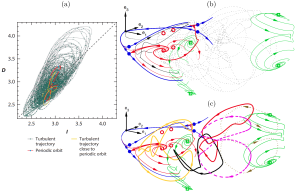
\includegraphics[width=\textwidth]{Background/Figures/BuildingBlocks.pdf}
    \caption{(a) Chaotic trajectories of turbulence of plane Couette flow at $Re = 400$, approaching the an unstable periodic orbit (red) highligted as yellow, adopted from \protect\cite{kawahara_periodic_2001}. (b) State space organisation of turbulence trajectores (black dots) confined around equilibria (circles, dots and squares) and their unstable manifolds (solid lines), heteroclinic connections between them are shown in red. The coordinate system, $(e_{1,2,3})$, is centered on the laminar state, using a linear combination of the upper branch invariant state. (c) State space projection of five periodic orbits (coloured solid lines), embedded within the same space where turbulence evolves in (b), adopted from \protect\cite{cvitanovic_geometry_2010}.}
    \label{fig:BuildingBlocks}
\end{figure}

A major development came with the identification of a pair of non-trivial, unstable equilibrium states in plane Couette flow \citep{nagata_three-dimensional_1990}.
This pair referred to as the \textit{lower} and \textit{upper} branches, emerging from a saddle node bifurcation disconnected from the stable laminar state.
% In the context of parallel shear flows, Nagata was the first to discover a pair of unstable equilibirum solutions in plane Couette flow by smoothly following (homotopy) from a Taylor-Couette configuration \citep{nagata_three-dimensional_1990}.
% This pair consist of an unstable upper branch and lower branch emerging as a saddle-node bifurcation near $Re \approx 500$, and is disconnected from the stable laminar solution.
The \textit{lower} branch lies closer to the laminar state, while the \textit{upper} branch resides further away in state space.
% The lower branch refers to its proximity towards the stable laminar state in phase space.
Later, a travelling-wave solution in plane Couette flow also later found by the same author \citep{nagata_three-dimensional_1997}.
A family of equilibrium and travelling-wave solutions was found later for plane Couette and plane Poiseuille flows under different boundary conditions (i.e. stress-free, slip and no-slip) were identified by \citep{waleffe_exact_2001,waleffe_homotopy_2003}.
Additional equilibria and travelling-wave solutions were identified by \cite{gibson_visualizing_2008,gibson_equilibrium_2009}, along with their heteroclinic connections between them \citep{halcrow_heteroclinic_2009}.
In the context of pipe flow, multiple travelling-wave solutions have also been reported 
\citep{faisst_traveling_2003,wedin_exact_2004,kerswell_recurrence_2007,wang_lower_2007,duguet_transition_2008,pringle_highly_2009}.
The set of equilibria, and travelling waves, shows good agreement with the statistical quantities (e.g. mean and fluctuations) with direct numerical simulations.
However, since they time independent (within a moving reference frame for travelling waves), they do no capture the temporal dynamics of turbulence such as the \textit{self-sustaining process} (SSP) \citep{hamilton_regeneration_1995} (see \S \ref{subsec:SSP}).
While these unstable solutions demonstrate good agreements with results from DNS such as the spanwise length scales, and mean and fluctuations, they do not capture the dynamical processes.


The next breakthrough was on the idenfitification of time-dependent unstable solutions in the form of periodic orbits. 
\cite{kawahara_periodic_2001} computed a pair of periodic orbits in plane Couette, with one exhibiting a single regeneration cycle similar to the SSP (see figure \ref{fig:BuildingBlocks}(a)) while the other exhibits mild modulation of streaks.
These periodic orbits are linked by heteroclinic connections.
In plane Poiseuille flow, \cite{toh_periodic-like_2003} also identified periodic orbits displaying bursting behaviour.
Using a Newton–Krylov iteration with a hook-step modification, \cite{viswanath_recurrent_2007} computed multiply relative periodic orbits.
These studies conceptualise that the chaotic trajectories of turbulence as being embedded within a set of unstable periodic orbits, evolving along their unstable manifolds \citep{viswanath_recurrent_2007,gibson_visualizing_2008,gibson_equilibrium_2009,halcrow_heteroclinic_2009,graham_exact_2021}.
An example is shown in figure \ref{fig:BuildingBlocks}, where the chaotic trajectories in figure \ref{fig:BuildingBlocks}(b), reside within the same state space as the periodic orbits, enclosed by equilibria and their heteroclinic connections shown in figure \ref{fig:BuildingBlocks}(c),
The set of equilibria, travelling waves and their relative counterparts, are referred to as \textit{invariant solutions} offering a building block description of turbulence.
However, they do not provide insight into the transition process, since these solutions already reside in the turbulent attractor.

\begin{figure}[h]
    \centering
    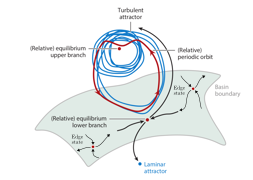
\includegraphics[width=0.8\textwidth]{Background/Figures/EdgeStates.pdf}
    \caption{A graphical representation of the edge (grey surface) separating the basin of boundary of the laminar and turbulent attractor, consisting of attractors, known as edge states, adapted from \protect\cite{graham_exact_2021}.}
    \label{fig:EdgeStates}
\end{figure}
The transition to turbulence in canonical shear flow configurations are typically subcritical, emerging from the invariant solutions described above, accompanied by an underlying stable laminar state.
A consequence of this is that the laminar and turbulent states form a bistable attractors in phase space with a boundary, separating their respective basins of attraction known as the \textit{edge}.
Attractors that sit along this edge have been identified and found to possess a saddle-like structure, attracting trajectories within the edge and repelling them toward either the laminar or turbulent state, known as \textit{edge} states.
The bisection algorithm used for edge tracking, was first employed in pipe flow experiments by \cite{schneider_turbulence_2007}, was identified to be chaotic.
Time-averaging of this chaotic attractor revealed a close resemblance to the unstable lower branch travelling-wave solutions, suggesting that the edge separating basin of attraction between the laminar and turbulent states consist of the lower branch solutions and their symmetries \citep{duguet_transition_2008,pringle_highly_2009}.
As Reynolds number increases, the edge and the turbulent attractor moves apart \citep{schneider_edge_2009}.
In the context of pipe flows, it was recognised that the edge consists of a set of unstable lower branch travelling-wave solutions.
A graphical representation of the edge, and edge states, separating the laminar the turbulent states is shown in figure \ref{fig:EdgeStates}.

\textcolor{red}{Near} the onset of subcritical turbulence, turbulence appear to be transient, decaying towards the laminar solution after a finite lifetime \citep{bottin_discontinuous_1998,faisst_sensitive_2004,hof_finite_2006}
% \red{This is often interpreted as the turbulent chaotic attractor colliding with the lower branch solution through a \textit{boundary crisis} \citep{lai_transient_2011}, where the chaotic attractor becomes \textit{leaky}, providing a pathway towards relaminarisation observed in pipe flows \citep{mellibovsky_travelling_2012}, plane Coutte flow \citep{kreilos_periodic_2012} and plane Poiseuille flow \citep{zammert_crisis_2015}.}
% \red{This is often interpreted as the turbulent chaotic attractor colliding with the lower branch solution through a \textit{boundary crisis} \citep{lai_transient_2011}, where solution trajectories may `leak' (relaminarise) towards the laminar state in pipe flows \citep{mellibovsky_travelling_2012}, plane Couette flow \citep{kreilos_periodic_2012} and Poiseuille flow \citep{zammert_crisis_2015}.}
This can be interpreted as the turbulent chaotic attractor colliding with the lower branch solution through a \textit{boundary crisis} \citep{lai_transient_2011}, forming a chaotic saddle where solution trajectories may `leak' (relaminarise) towards the laminar state \citep{mellibovsky_travelling_2012, kreilos_periodic_2012, zammert_crisis_2015}.
The onset a boundary crisis (transient turbulence) have been also attributed to the emergence of homoclinic tangency in plane Couette flow \citep{van_veen_homoclinic_2011,lustro_onset_2019}.
% where solutiont trajectories could leak towards the laminar state after spending a considerable amount of time in the turbulent attractor.
% wandering around the set of invariant solutions along the edge, before falling back onto the laminar state.

% Turbulent trajectories to appear to be embedded within a collection of unstable periodic orbits, evolving along their unstable manifolds \citep{viswanath_recurrent_2007, gibson_visualizing_2008}
% These studies conceptualise chaotic turbulent trajectories as being embedded within a set of unstable periodic orbits, evolving along their unstable manifolds \citep{viswanath_recurrent_2007,gibson_visualizing_2008,gibson_equilibrium_2009,halcrow_heteroclinic_2009,graham_exact_2021}.

% Chaotic trajectories appear to be embedded within a network of unstable periodic (and relative periodic) orbits and their heteroclinic connections.

% The chaotic trajectories of turbulence have been found to be embedded within invariant solutions and their connections between them known as heteroclinic orbits, offering a robust view of the building-blocks of of turbulence \citep{gibson_visualizing_2008, gibson_equilibrium_2009, viswanath_recurrent_2007, halcrow_heteroclinic_2009, graham_exact_2021}

% In the context of this transitional flows, the lower branch solution can be though of separating the turbulent attractor from the laminar state.
% Its an attractor that resides on the edge of turbulence, defined as an edge state.
% The graphical representation of this edge is shown in figure \ref{fig:StateSpaceGraham}.

% Coherent structures and turbulent motions
% These invariant solutions commonly take the form of as equilibria, travelling waves, periodic and relative periodic orbits.
% It is well established that coherent motions defined by flow patterns that persist in space and time play an important role in the transport of momentum and heat.
% In parallel shear flows, these coherent structures typically appear as near-walls streaks and quasi-streamwise rollers.
% A persistent, quasi-periodic cycle between the regeneration of streaks and rolls, referred to as the \emph{self-sustaining process}, appears to be a fundamental mechanism in sustaining wall-bounded turbulence \emph{self-sustaining process} \citep{hamilton_regeneration_1995}.
% This mechanism is described by the generation of streaks due to quasi-streamwise rollers by redistributing the mean.
% These streaks become linearly unstable and breakdown, and through a nonlinear process regenerates the quasi-streamwise rollers, closing the cycle.

% Utilising tools from nonlinear dynamics systems, turbulence could be viewed as chaotic trajectories around unstable nonlinear solutions known as invariant solutions or exact coherent structures \citep{Waleffe_2001,Waleffe_2003,toh2003periodic,Kreilos_2012,nagata2013mirror,Wall_Nagata_2016,Zammert_Eckhardt_2014,graham21}.

%%%%%%%%%%%%%%%%%%%%%%%%%%%%%%%%%%%
% The self-sustaining process 
%%%%%%%%%%%%%%%%%%%%%%%%%%%%%%%%%%%
\subsection{Self-sustaining process}\label{subsec:SSP}
\begin{figure}[h]
    \centering
    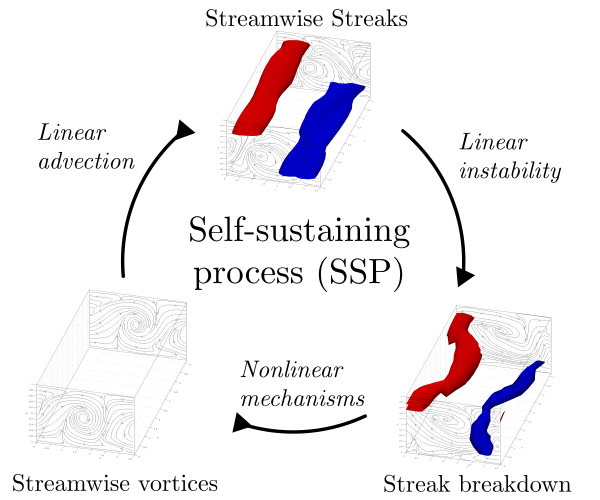
\includegraphics[width=0.7\textwidth]{Background/Figures/SSP/SSP.pdf}
    \caption{The self-sustaining process, consisting of three phases: (1) Streak formation from linear advection by streamwise vortices, (2) streak breakdown due to streak instability and (3) regeneration of streamwise vortices via nonlinear mechanisms.}
    \label{fig:SSP}
\end{figure}

The self-sustaining process (SSP) describe the dynamical interaction between a pair of streaks and quasi-streamwise vortices, considered to be the fundamental process of wall bounded turbulent flows in the near wall region.
It is defined by a quasi-cyclic process, consisting of three distinct phases: (1) the formation of streamwise streaks due to a linear advection by streamwise vortices, (2) the wavy breakdown of streaks due to linear instability and (3) the regeneration of streamwise vortices via nonlinear mechanisms \citep{durst_origin_1993,waleffe_self-sustaining_1997,hamilton_regeneration_1995}.
A schematic of the SSP is shown in figure \ref{fig:SSP}.
While early investigations of the SSP was confined the buffer layer \citep{hamilton_regeneration_1995}, evidence that the SSP extends towards the logarithmic and outer region has been found \citep{cossu_self-sustaining_2017}.
In parallel to the SSP, the vortex-wave interaction (VWI) theory developed to describe the sustained interactions between a general class of vortices and waves for asymptotically large Reynolds number \citep{hall_nonlinear_1988,hall_strongly_1991,stewart_near-planar_1990}, was found to be linked to the SSP \citep{hall_streamwise_2010}.
In particular, the solutions obtained using VWI theory by \cite{hall_streamwise_2010} is analagous to the lower branch solution from \cite{wang_lower_2007}.

%%%%%%%%%%%%%%%%%%%%%%%%%%%%%%%%%%%
% Spatiotemporal transitional flows
%%%%%%%%%%%%%%%%%%%%%%%%%%%%%%%%%%%

\subsection{Spatiotemporal transitional flows}
\begin{figure}[h]
    \centering
    \includegraphics[width=\textwidth]{Background/Figures/Re1400.pdf}
    \caption{A snapshot of turbulent-laminar bands at $Re = 1400$ in a large domain $L/h = 16\pi$, depecting its spatiotemporal intermittent nature. Isovolume renderings is based on the spanwise, $u'$, and wall-normal, $v'$, perturbation kinetic energy, $E(u',v') = 1/2(u'^2 + v'^2)$, where the perturbation velocities are defined about the laminar state $\mathbf{u}'(\mathbf{x},t) = \mathbf{u}(\mathbf{x},t) - U_{lam}(y)$.}
    \label{fig:turbulent-laminar}
\end{figure}

This section describes the inherent spatiotemporal structure of subcritical turbulence near the onset commonly reported in large extended domains.
% where the span is about fifty times the half-height of a plane Poiseuille channel, $L/h \gtrsim 50$.
In this regime, turbulence is characterised by the coexistence of turbulent and laminar structures.
Examples of such are found in canonical shear flow systems such as plane Couette flows \citep{prigent_long-wavelength_2003,barkley_computational_2005,barkley_mean_2007,tuckerman_patterns_2011,duguet_formation_2010,reetz_exact_2019}, Taylor-Couette flows \citep{prigent_barber_2002,prigent_long-wavelength_2003}, pipe flows \citep{avila_transient_2010,avila_onset_2011,song_speed_2017,avila_transition_2023} and plane Poiseuille flows \citep{tsukahara_dns_2014, tsukahara_dns_2014-1, tuckerman_turbulent-laminar_2014, tsukahara_experimental_2014, gome_statistical_2020, paranjape_onset_2019, paranjape_oblique_2020, paranjape_direct_2023}.

We will focus on the plane Poiseuille flow configuration, where the spatiotemporal intermittent patterns are referred to as oblique turbulent-laminar bands illustrated in figure \ref{fig:turbulent-laminar} at $Re = 1400$ for $L/h = 16\pi$.
The bright and dark regions highlights coexisting spatially localised turbulent and laminar regions.
These turbulent-laminar bands occur over a range of Reynolds numbers, and its precise range is dependent on the domain's aspect ratio \citep{tsukahara_experimental_2014,tuckerman_turbulent-laminar_2014,paranjape_direct_2023}.
Near the upper $Re$ threshold of this regime, the domain is fully engulfed by uniform, featureless turbulence appearing at $Re = 1800$ in figure \ref{fig:turbulent-laminar}(a).
As $Re$ decreases towards $Re = 1050$, spatiotemporal turbulent and laminar structures known as turbulent-laminar bands persist in between $Re \in [1050, 1600]$ shown in figures \ref{fig:turb_lam_bands}(b-f).
In particular, these turbulent-laminar appear to have a preferred inclined angle, between $20^\circ \sim 30^\circ$, with streamwise wavelengths of $\lambda_x \sim 60h$, and spanwise wavelengths of $\lambda_z \sim 20h-30h$ \citep{tsukahara_experimental_2014}.
\cite{kashyap_linear_2022} considered the linear response of the fluctuating turbulent field, and showed that the preferred band angle emerges near $23.2^\circ$.
% Inspired from previous studies of turbulent-laminar bands in plane Couette flows \citep{barkley_computational_2005, reetz_exact_2019}, the minimal band unit (MBU) was employed for plane Poiseuille flows \citep{tuckerman_turbulent-laminar_2014, paranjape_oblique_2020, paranjape_direct_2023}.
% In MBUs of plane Poiseuille flows, the turbulent-bands convect at about $\sim1\%$ of the bulk velocity, propagating either upstream or downstream, above or below an critical $Re \sim 1000$, independent of domain sizes for $L_z \geq 100h$ \citep{tuckerman_turbulent-laminar_2014,gome_statistical_2020}.
In the minimal band unit (MBU) studies of plane Poiseuille flows, the turbulent-bands convect at about $\sim1\%$ of the bulk velocity, propagating either upstream or downstream, depending on $Re$ \citep{tuckerman_turbulent-laminar_2014,gome_statistical_2020}.
% To study the preference of angles, zzz performed linear stability analysis of bands and showed that preferred angle at .. degrees.
Notably, the spanwise lengths of the bands are much wider than the half-heights and depends on $Re$, appearing at $\lambda_z \sim 20h$ for $Re \gtrsim 1400$ and $\lambda_z \sim 40h$ for $Re \lesssim 1100$.
Interestingly, the bands alternate between both spanwise lengths between the $Re$ range, merging and splitting continuously \citep{tuckerman_turbulent-laminar_2014}, reminiscent of a puff splitting process in pipe flows \citep{avila_onset_2011}.
An example of this could been observed in $Re = 1050$, where the band appears to alternate between different spanwise wavelengths in figure \ref{fig:turb_lam_bands}(f).
% Below certain $Re$ threshold, the spatially turbulent regions decay where the flow relaminarises \citep{tuckerman_turbulent-laminar_2014}.
As $Re$ falls below a certain $Re$ threshold, turbulent bands spontaneously decay and relaminarises \citep{tuckerman_turbulent-laminar_2014,gome_statistical_2020}.
An example is shown in figure \ref{fig:turb_lam_bands}(g).
% An example of this decay is shown in $Re = 1000$ near $t = 1600$ in figure \ref{fig:turb_lam_bands}(g). 
\begin{figure}[h]
    \centering
    \includegraphics[width=\textwidth]{Background/Figures/Ra0-BotSpaceTime.pdf}
    \caption{Turbulent-laminar bands for $t \in [0, 3000]$ in large domains $(L_x, L_z) = (16\pi, 16\pi)$ at (a) $Re = 1800$, (b) $Re = 1600$, (c) $Re = 1400$,  (d)  $Re =1200$, (e) $Re = 1100$, (f) $Re = 1050$,  (g) $Re = 1000$.}
    \label{fig:turb_lam_bands}
\end{figure}

\begin{figure}[h]
    \centering
    \includegraphics[width=0.7\textwidth]{Background/Figures/gome_prob.pdf}
    \caption{The mean decay times (red), $\tau^d$, and mean splitting times (black), $\tau^s$, as a function of Reynolds number, leading to a crossover point at $Re_{cross} \approx 965$, adapted from \protect\cite{gome_statistical_2020}.}
    \label{fig:decay_split_probability}
\end{figure}

% As $Re$ is lowered turbulent bands appear to decay at $Re = 830$ \citep{gome_statistical_2020}, and at $Re = 1100$ but surviving for $Re = 1000$ \citep{tuckerman_turbulent-laminar_2014}, suggesting that turbulent bands decay spontaneously.
% However, at $Re = 1100$ but surviving for $Re = 1000$ \citep{tuckerman_turbulent-laminar_2014}, suggesting that turbulent bands decay spontaneously.
\cite{gome_statistical_2020} computed the \textcolor{red}{probability} distributions for turbulent-laminar band decay, $P(\Delta t^d)$, where $\Delta t^d$ is the time until decay.
A key insight is that the probability distributions of turbulent band decay mimics a memoryless Poisson process,
\begin{equation}
    P(\Delta t^d) = \exp(-\Delta t^d/\tau^d(Re)),
\end{equation}
where $\tau^d(Re)$ refers to the mean lifetime for decay as a function of $Re$.
Similarly, the band splitting process also follow a Poisson process,
\begin{equation}
    P(\Delta t^s) = \exp(-\Delta t^s / \tau^s(Re)),
\end{equation}
\textcolor{red}{where $\tau^s(Re)$ refers to the mean splitting lifetime.}
% the probability distribution for band splitting also follows a Poisson distribution, , where $\tau^s(Re)$ refers to the mean lifetime of a splitting event dependent on $Re$.
Both $\tau^d$ and $\tau^s$ exhibit superexponential dependence on $Re$,
\begin{equation}
    \tau^{d,s} = \exp(\exp(Re)),
\end{equation}
% The mean survival lifetime of a band decaying, $\tau^d$, and splitting, $\tau^s$, depends superexponentially on $Re$, i.e. $\tau^{d,s} = \exp(\exp(Re))$.
This is shown in figure \ref{fig:decay_split_probability}, with a crossover point at $Re_{cross} \approx 965$, where both decay and splitting becomes equally probable.
This crossover point is considered as the critical Reynolds number for the onset of turbulent bands.
% By extrapolating the estimated mean lifetimes of a splitting and decay event, the crossing point (i.e equal chance of identifying a splitting and decay event after a time-scale of $t = 3 \times 10^6$) occurs at $Re_{cross} \approx 965$, in other words, $Re_{cross}$ acts as a critical Reynolds number.

While there has been progress made towards our understanding of infinitely bi-periodic turbulent-laminar bands in MBUs, recent studies of isolated (non-periodic) turbulent bands (ITBs) reveal different behaviour.
Notably, ITBs persist at Reynolds number below $Re_{cross}$ at $Re = 700$ for durations \textcolor{red}{of} $t = 10000$, exceeding the mean decay lifetime in figure \ref{fig:decay_split_probability}.
The ITBs are characterised by \textcolor{red}{a} streak generating head and a diffusive upstream tail. \citep{xiong_turbulent_2015, tao_extended_2018, shimizu_bifurcations_2019, xiao_growth_2020}.
\textcolor{red}{Here,} we conclude our discussion  on transitional wall-bounded shear flows.
% It is worth noting that isolated bands are not memoryless, depending on their pass history [citation]
% Above a certain Reynolds number, the probability of band splitting again depends on a super-exponentianal.
% Show graph.
% In the context of plane Poiseuille flowsd, it is well known that at $Re \sim 1000 - 2000$, turbulence behaves intermittently, existing as oblique bands of turbulent and laminar regions. 
% Over the past decade, research efforts have been dedicated to the study of turbulent-laminar bands.

% At $Re \sim 1000 - 2000$, turbulent bands can either decay spontaneously, stabilising into a laminar state, or split, forming more bands whereby turbulent-laminar bands are sustained.
% The probability of decay and splitting lifetimes strongly depends on the domain size and $Re$.
% At $L_z = 100h$, the critical Reynolds number of $Re_{cr} \approx 965$ have been determined statistically, whereby decay and splitting lifetimes intersect more than $10^6$ advective time units. 
% It is worth to note that for $Re < Re_{cr}$, the probably of decay is higher than splitting events, vice versa. 


%%%%%%%%%%%%%%%%%%%%%%%%%%%%
% Rayleigh Benard Convection
%%%%%%%%%%%%%%%%%%%%%%%%%%%%

\section{Rayleigh-B\'{e}nard convection}\label{sec:bkgrd_RBC}

\begin{figure}[h]
    \centering
    \includegraphics[width=\textwidth]{Background/Figures/BenardCells.png}
    \caption{(a) Surface tension driven convection leading to the onset of hexagonal B\'{e}nard cells in a thin layer of silicone oil, heated from below and cooled by ambient air. A diamond defect appears, likely caused by plate imperfections. (b) Buoyancy driven convection in rigid plates, resulting to concentric convection rolls at $2.9$ times the critical Rayleigh number. Both experiments were performed by \protect\cite{koschmieder_heat_1974}, and the convection patterns were illuminated by aluminum powder, where the dark and bright regions refer to vertical and horizontal motions resepctively. These higher resolution images were taken from \protect\cite{van1982album}.}
    \label{fig:benard_cells}
\end{figure}

Rayleigh-B\'{e}nard convection (RBC) is a paradigmatic fluid configuration describing the motion of the fluid confined between two infinite-parallel plates heated from below and cooled from the top.
% The basic physical mechanism underpinning RBC is variation of buoyancy due to heat, offering a simple description of natural convection.
As the bottom plate is heated, the bottom layer fluid becomes more buoyant and tends to rise, while the colder top fluid layer \textcolor{red}{becomes} relatively less buoyant and tends to sink, leading to an overturning of layers \textcolor{red}{leading to motion.}
Viscous forces between neighbouring fluid parcels act to resist \textcolor{red}{this} motion. 
As buoyancy overcomes these viscous forces, the fluid layers overturn, resulting in \textcolor{red}{fluid motion and the initiation of buoyancy-driven convection, the physical mechanism underpinning RBC.}

One of the earliest experimental studies dedicated to buoyancy-driven convection was conducted by Henri B\'{e}nard \citep{benard_tourbillons_1901}, who observed the formation of hexagonal convection cells above a certain temperature threshold $\Delta T$.
These hexagonal patterns are referred to as B\'{e}nard cells are illustrated in figure \ref{fig:benard_cells}(a) (adapted from \citep{koschmieder_heat_1974}).
Subsequently, \cite{rayleigh_lix_1916} carried out one of first linear stability analyses of buoyancy-driven convection, predicting the onset of convection at a critical Rayleigh number of $Ra_c = 657.5$.
However, Rayleigh's analysis assumed an idealised free-free boundary conditions, which differed from the rigid-free setup of B\'{e}nard's experiment.
The linear stability analysis for rigid-free configuration was later performed by \cite{jeffreys_cases_1928} yielding a higher critical Rayleigh number of $Ra_c = 1058$.
In the rigid-rigid configuration, the critical Rayleigh number increases further to $Ra_c = 1708$ \citep{pellew_maintained_1940}.
The Rayleigh number in B\'{e}nard's original experiment contradicted results from linear stability analysis as it was found to be 300 to 1500 smaller than $Ra_c$ for the free-free and rigid-free cases respectively \citep{wesfreid_henri_2017}.
% However, it is worth highlighting a key difference in B\'{e}nard's experiment and Rayleigh's analysis.
This contradiction, not recognised by B\'{e}nard at the time, lies in the significant role of surface tension \textcolor{red}{of} thin fluid layers exposed to air, now known as \textcolor{red}{B\'{e}nard-Maragoni convection (BMC)} \citep{block_surface_1956, cloot_nonlinear_1984, hohler_rayleigh-benard_2006, wesfreid_henri_2017}.
In \textcolor{red}{BMC}, fluid motion is primarily driven by surface tension gradients due to variations of temperature, forming hexagonal cells, as in figure \ref{fig:benard_cells}(a).
The preference for hexagonal cells in \textcolor{red}{BMC} was later confirmed based on weakly nonlinear stability analysis \citep{cloot_nonlinear_1984}.
% as in B\'{e}nard experiments, a thin layer of fluid exposed to the air is chiefly driven by the variation of surface tension due to temperature difference, leading to the growth of hexagonal cells, in figure \ref{fig:benard_cells}(a).
As the fluid layer becomes thicker, surface-tension effects diminish and buoyancy-driven convection becomes dominant.
Similarly, placing a rigid lid on top of a thin fluid layer suppresses surface-tension effects, resulting in buoyancy-driven convection. 
\textcolor{red}{The difference between RBC an \textcolor{red}{BMC} is shown in \ref{fig:benard_cells}.}
% Surface-tension effects diminish as the fluid depth increases, or removed in the presence of a top rigid lid, where buoyancy becomes the dominant mechanism.
The preferred convection patterns of \textcolor{red}{RBC} based on weakly nonlinear stability analysis are the two-dimensional parallel rolls, now referred to as ideal straight rolls (ISRs) \citep{schluter_stability_1965, bodenschatz_recent_2000}.
% This also have the same effect as placing a lid on top of thin layer of fluid where surface-tension effects are removed, leading to ISRs.
% This key discrepancy was later identified as B\'{e}nard's experiments considered thin layers of fluid heated and cooled by the ambient air \citep{block_surface_1956}, where surface tension (Maragoni) effects were significant.
In circular \textcolor{red}{containers, ISRs} conform to the geometry of the boundaries, forming concentric convection rolls illustrated in figure \ref{fig:benard_cells}(b).
Interestingly, hexgaonal cells have been observed in buoyancy-driven flows of non-Boussinesq fluids \citep{hoard_experiments_1970,bodenschatz_recent_2000}.
In this thesis, we consider the RBP setup (and RBC in chapter 4) with rigid-rigid boundary conditions, bearing \textcolor{red}{the} critical Rayleigh number of $Ra_c = 1708$.
Notably, the corresponding critical wavelength is $q_c = 3.12 / d$ (or $\lambda_c \approx  2d$), suggesting that distance separating the plates, $d$, dictates the length of a single roll, $l_{roll} = \lambda_c / 2 \approx d$.
% 1. Bousinessq fluids (silicon oil) leads to 2D rolls or Hexagonal rolls for rigid-rigid and open-rigid B.Cs - highlighting the importance of the top B.C
%     a. Are they buoyancy driven or surface-tension driven?
% 
% 2. Non-bouseinessq (Aroclor) lead to rigid-rigid boundary conditions lead to rolls for thick layers, and hexes in thin layers. In open-rigid boundary conditions, 2D concentric rolls develop in thick layers while hexagonal cells form in thin layers.


% While the $Ra_c$ for free-free and rigid-free have been reported \citep{rayleigh_lix_1916,jeffreys_cases_1928}.
% It is also worth noting that \cite{rayleigh_lix_1916} considered a stress-free boundary conditions in his analysis, which has been extended to rigid boundary conditions, the critical Rayleigh number increased to well known $Ra_c = 1707.8$ \citep{pellew_maintained_1940}, and is independent or $Pr$ \citep{bodenschatz_recent_2000}.

% ension decreases  generated a tangential forces towards regions of higher surface tension at the surface, where cold fluid resides, ampliying convection, now known as B\'{e}nard-Maragoni convection \citep{manneville_thirty_2006}. 
%, with a critical wavenumber of $q_c = \frac{\pi}{\sqrt{2}d}$.
% and predicted the critical Rayleigh number of $Ra_c = \frac{27}{4}\pi^4 = 657.5$, and a critical wavelength of $q_c = \frac{\pi}{\sqrt{2}d}$.
% where $Ra, \alpha, g, d \Delta T, \kappa, \nu$ refers to the Rayleigh number, volumetric thermal expansion of the fluid, gravitational constant, width and temperature difference between plates, thermal diffusivity and kinematic viscosity. 
% When $Ra$ exceeds a certain critical Rayleigh number $Ra_c$, the fluid configuration becomes unstable and convection motion ensures.
% The pioneering work from Rayleigh, and B\'{e}nard's experiment formed the early foundations of buoyancy-driven convection, now known as Rayleigh-B\'{e}nard convection.
% In the absence of surface tension effects, the critical Rayleigh number, $Ra_c$ depends on the boundary condition, commonly analysed using stress-free or rigid-rigid (no-slip) boundary conditions.
% In Rayleigh's work, he considered a stress-free condition at the wall, ${\partial u}/{\partial n} = 0$, where analytical solutions are admittable.

\begin{figure}[t]
    \centering
    \includegraphics[width=0.8\textwidth]{Background/Figures/BusseBalloonFull.png}
    \caption{The Busse ballon describes the stability boundaries of ISRs in a $\varepsilon-q$ space. For larger wavenumbers, the instability mechanisms is described by the skewed-varicose (SV) instability. For smaller wavenumbers, the instability mechanism is described by the Eckhaus instability. For large $\varepsilon$, the instability is described by the onset of oscillatory instability. Busse balloon digitised from \protect\cite{plapp_spiral_1997} for $Pr \approx 1$.}
    \label{fig:busseballon}
\end{figure}

% As mentioned earlier, stationary ISRs near $q_c$ emerge just above $Ra_c$, based on weakly nonlinear stabity analysis. \citep{eckhaus_studies_1965, schluter_stability_1965}.
\textcolor{red}{While weakly nonlinear analysis predicts the onset of stationary ISRs, the emergence of time-dependent oscillatory ISRs in experiments \citep{rossby_study_1969,willis_oscillatory_1970} at $Ra = 9200$ (or roughly five times $Ra_c$), contradicts the analysis which likely becomes inapplicable far from threshold.}
To address this, a secondary stability analysis was \textcolor{red}{performed} to study the stability of ISRs further from $Ra_c$ \citep{busse_oscillatory_1972}.
% \cite{busse_oscillatory_1972} performed secondary linear stability analysis of ISRs based on Galerkin truncation of orthogonal functions.
One of the key results from this analysis is the Busse balloon, which describes the stability boundaries of ISRs as a function of $Ra$ and $Pr$, and roll wavenumber, $\alpha$, shown figure \ref{fig:busseballon} \citep{busse_non-linear_1978}.
The boundaries of the Busse balloon are described by a range of secondary instabilities, each arising from different physical mechanisms \citep{busse_non-linear_1978}.
At large Prandtl numbers, $Pr = O(10^2)$, the zig-zag (ZZ) and cross-roll (CR) instabilities delimits the balloon for small and large roll wavenumbers.
The zig-zag instabilities cause zig-zag undulations while the CR instabilities generates rolls orthogonal to the underlying ISR structure, effectively increasing or decreasing the roll wavenumber respectively \citep{busse_instabilities_1971}.
Examples of these instabilities at $Pr = 100$ are illustrated in figure \ref{fig:busseballoon_secinstab}(a,b).

\begin{figure}
    \centering
    \includegraphics[width=0.5\textwidth]{Background/Figures/BusseBalloon/SecondaryInstabilities.pdf}
    \caption{ISRs experiencing (a) cross-roll instability at $Ra = 3000, Pr = 100$ and (b) zig-zag instability at $Ra = 3600, Pr = 100$ \protect\citep{busse_instabilities_1971}. (c) Skew-\textcolor{red}{varicose} instability at $Ra = 5568, Pr = 1$ \protect\citep{plapp_spiral_1997}, and (d) oscillatory instability at $Ra = 10384, Pr = 1$ \citep{cakmur_bistability_1997}.}
    \label{fig:busseballoon_secinstab}
\end{figure}

At moderate Prandtl numbers, $Pr = O(1)$, the Busse balloon is bounded by the skewed \textcolor{red}{varicose} (SV) for high roll wavenumbers and the oscillatory (OS) instability at large $Ra$.
% The cross-roll instability generates an additional roll orthogonal to the existing roll, while the zig-zag instabilities leads to the emergence of zig-zag ISRs.
The skewed-\textcolor{red}{varicose} (SV) instability leads to roll-pinching where pinched rolls merged into a single roll, reducing roll wavenumber while the oscillatory instability leads to the onset of an oscillatory ISRs. 
Examples of the respective instabilities at $Pr = 1$ are shown in figure \ref{fig:busseballoon_secinstab}(c,d).
At higher wavenumbers, the skewed varicose (SV) instability becomes relevant at intermediate Prandlt numbers, characterised by roll pinching and merging that effectively reduces the roll wavenumber.
% For larger Rayleigh numbers and $Pr \lesssim 1$, the oscillatory instability (OS) arises, forming oscillatory ISRs \citep{willis_oscillatory_1970}.
% In contrast, for higher $Pr$, the knot instability appears, modifying the cross-roll pattern into a spoke-like structure.
Finally, the Eckhaus instability (not shown), related to the symmetry of the system, appears close to the $Ra_c$, leading a disturbance parallel to the underlying rolls which either creates or destroy rolls such that the resultant roll wavenumber adheres to the stability boundaries \citep{lowe_pattern_1985}.
Near $Pr = 1$, the Eckhaus instability coincides with the crossroll instability (figure 6 from \cite{bodenschatz_recent_2000}, adapted from \cite{plapp_spiral_1997}.)

In this thesis, we focus on fluids with $Pr = 1$, where secondary instabilities such as \textcolor{red}{the} skewed-varicose, Eckhaus and cross-roll instabilities typically arise.
While the stability boundaries of the Busse balloon have been experimentally verified \citep{busse_instabilities_1971, croquette_convective_1989, plapp_spiral_1997}, \textcolor{red}{predicting} the wavenumber of ideal straight rolls (ISRs) remain difficult due to hysteresis and the existence of multiple stable ISRs of different roll wavenumbers.
As $Ra$ continously increases, ISRs with wavenumbers outside the Busse Balloon undergo the secondary instabilities that \textcolor{red}{modify} their wavenumbers \textcolor{red}{to conform to} the stable boundaries.
% These instabilities either increase or decrease the roll wavenumber, adhering to the the stability boundaries of the Busse balloon.
The hysteretic behaviour highlights that the roll wavenumber of the ISRs is strongly dependent on the system's history \citep{bodenschatz_recent_2000}.

% MULTIPLE STATES
It is worth noting that the ISRs are the exception rather than the rule in RBC \citep{croquette_convective_1989-1}.
A range of non-ISR states, such as squares, travelling or stationary target patterns, giant rotating spirals, and oscillatory convection, have been observed over the years \citep{le_gal_square_1985, croquette_convective_1989, plapp_spiral_1997, hof_flow_1999, rudiger_pattern_2000, boronska_extreme_2010, boronska_extreme_2010-1}.
% The coexistence of multiple ‘non-ISR’ states, in the form of squares, travelling/stationary targets, giant rotating spirals, and oscillatory convection patterns have been found over several years \citep{le_gal_square_1985, croquette_convective_1989, plapp_spiral_1997, hof_flow_1999, rudiger_pattern_2000, boronska_extreme_2010, boronska_extreme_2010-1}.
For example, \cite{hof_flow_1999} identified eight stationary and two oscillatory state in cylinderical RBC with small aspect ratios at the same Rayleigh number.
These results were later verified in numerical simulations and bifurcation analysis, revealing up to twelve stable branches near the onset ($Ra \leq 2500$) and the potential for hundreds more as $Ra$ increases \citep{ma_multiplicity_2006,boronska_extreme_2010,boronska_extreme_2010-1}.
% Investigation of cylindrical RBC with small aspect-ratio ($\Gamma = 2$) found eight stationary states (at the same $Ra = 142000$), and two oscillatory states ($Ra > 14200$) \citep{hof_flow_1999}.
% These findings were later supported by numerical experiments and bifurcation analyses \citep{ma_multiplicity_2006, boronska_extreme_2010, boronska_extreme_2010-1}.
% In particular, bifurcation analyses performed by \cite{ma_multiplicity_2006}, revealed twelve stable branches in the form of symmetric and asymmetric convection rolls near onset ($Ra \leq 2500$), with the potential emergence of hundreds of branches at higher Rayleigh numbers, $Ra \leq 30000 $ \citep{boronska_extreme_2010-1}.

In larger domains ($\Gamma \geq 28$), giant rotating spirals were found and have been investigated \citep{plapp_core_1996, plapp_dynamics_1998}.
Experimental and numerical studies of RBC with varying sidewall boundary conditions (i.e. thermally insulating, conducting an no-slip) \citep{tuckerman_global_1988, siggers_dynamics_2003, paul_pattern_2003,boulle_bifurcation_2022}, non-Boussinesq convection \citep{bodenschatz_experiments_1992}, and rotational effects \citep{hu_convection_1997} were investigated, where multiple states were also reported.
In inclined RBC, \cite{reetz_invariant_2020, reetz_invariant_2020-1} identified up to sixteen stable and unstable invariant states, along with heteroclinic orbits connecting them.
These findings indicate that RBC support a rich variety of coexisting stables states beyond ISRs, resulting to a system with multiple stable states above the critical Rayleigh number.

\begin{figure}[h]
    \centering
    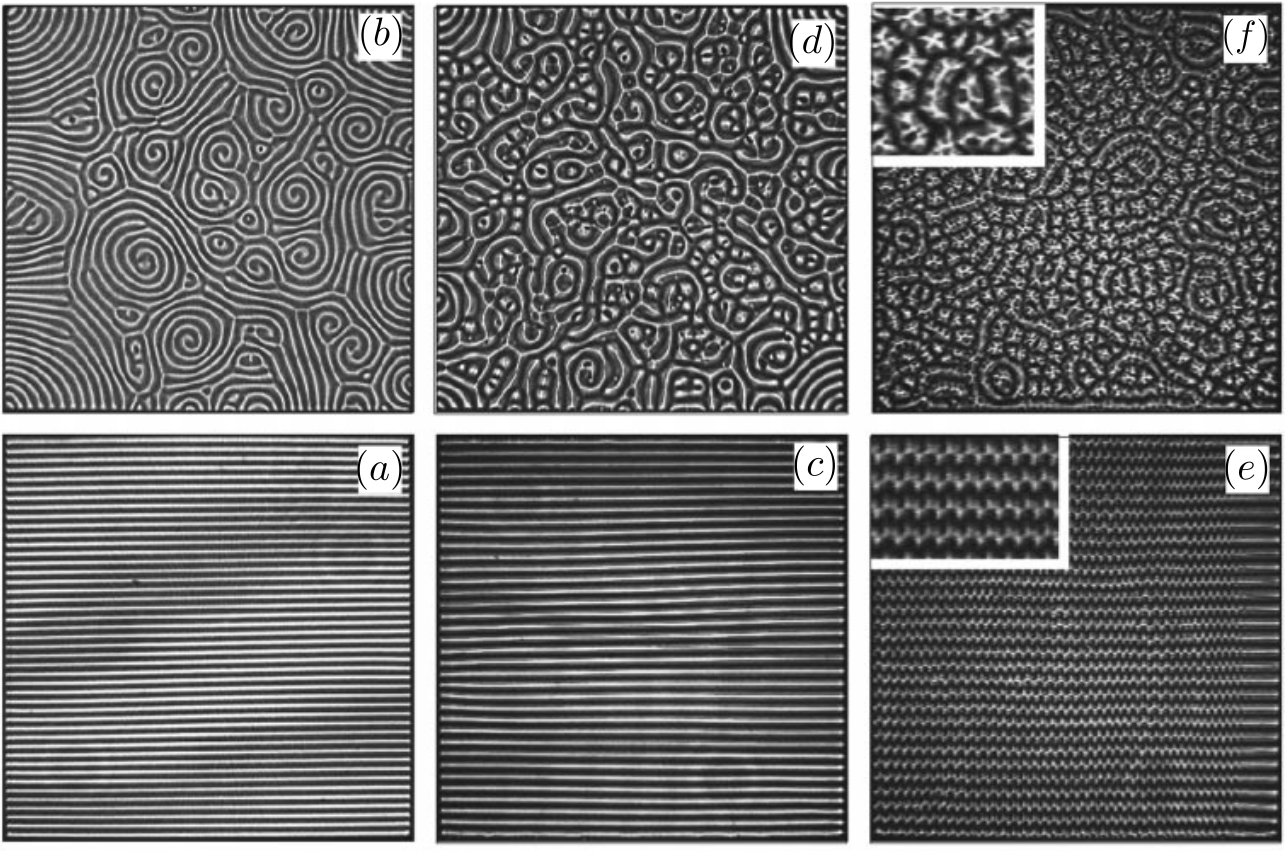
\includegraphics[width=0.8\textwidth]{Background/Figures/bistability.png}
    \caption{The coexistence of spiral defect chaos (SDC, top row) and ideal straight rolls (ISRs, bottom row) at (a,b) $Ra = 3279$, (c,d) $Ra = 6832$ and (e,f) $Ra = 10384$. The domain size is $\Gamma = 50$ and $Pr = 1$, adapted from \protect\cite{cakmur_bistability_1997}.}
    \label{fig:sdc_isr}
\end{figure}
% The existence of multiple stable states apart from ISRs suggest that RBC forms a multiple bistable systate above $Ra_c$.
% To compliate matter further, an instrinsic chaotic state of convection was discovered.

% SDC
\textcolor{red}{To complicate matters further, convection rolls exhibiting spatio-temporal chaotic behaviour known as spiral defect chaos (SDC) were discovered in the 1990s.}
\textcolor{red}{SDC was found within the same stability boundaries where ISRs were expected}\citep{morris_spiral_1993, hu_convection_1993,decker_spiral_1994,hu_convection_1995,morris_spatio-temporal_1996,cakmur_bistability_1997,ahlers_experiments_nodate,egolf_importance_1998,egolf_mechanisms_2000,chiam_mean_2003,vitral_spiral_2020}.
Notably, ISRs emerge with carefully prepared initial conditions while uncontrolled initial conditions lead to SDC.
It is now well established that SDC exists as intrinsic attractor of RBC, independent of sidewall conditions \cite{morris_spatio-temporal_1996}, forming a bistable system with ISRs \citep{cakmur_bistability_1997} across a range of $Ra$ at $Pr = 1$ illustrated in figure \ref{fig:sdc_isr}.
However, this bistability appears to be Prandtl number dependent. 
At $Pr = 4$, the SDC appears to be \textcolor{red}{transient, decaying} towards ISRs over long periods \citep{bajaj_competition_1997}.
SDC has also been replicated in numerical simulations using two-dimensional Swift-Hohenberg equations \citep{swift_hydrodynamic_1977,xi_spiral_1993,xi_spatiotemporal_1995,schmitz_spiral-defect_2002,karimi_exploring_2011}.
The critical Rayleigh number for the onset of SDC, $Ra_s$, depends on the domain's aspect ratio, and Prandtl number \citep{hu_convection_1995,bajaj_competition_1997,cakmur_transition_1997,bodenschatz_recent_2000}.
% Investigations into quantifying the onset of SDC in terms of Rayleigh number remain inconclusive as it appears to depend on the domain's aspect ratio, and Prandtl number \citep{hu_convection_1995,bajaj_competition_1997,cakmur_transition_1997,bodenschatz_recent_2000}.
% The critical reduced Rayleigh number for the onset of SDC, $\varepsilon_s$, has been observed to decrease with increasing $\Gamma$, and increase with increasing $Pr$ \cite{hu1995a, hu1995b, bajaj1997, Cakmur97, bodenschatz2000}.
SDC has been \textcolor{red}{reported} in large aspect ratio domains ($\Gamma \gtrsim 20$), suggesting a minimal domain size for SDC to occur \citep{bodenschatz_recent_2000}.
This is consistent with the leading Lyapunov exponents of SDC which becomes smaller with decreasing $\Gamma$ \citep{egolf_mechanisms_2000, paul_extensive_2007}.
To \textcolor{red}{characterise} SDC, several studies have investigated its spatial-temporal properties, such as the averaged roll-curvature \cite{hu_convection_1995}, probability distribution of spirals \cite{ecke_excitation_1995, liu_spiral-defect_1996} and correlation \textcolor{red}{length and time} scales \citep{morris_spiral_1993, morris_spatio-temporal_1996, cakmur_transition_1997}.
Specifically, the correlation length-scales were found to grow exponentially with \citep{morris_spiral_1993, morris_spatio-temporal_1996, cakmur_transition_1997}, suggesting that transition from ISRs to SDC is related to phase transitions.
Similar `SDC-liked' has been observed in other pattern-formation systems, including rotating RBC \cite{hu_convection_1997}, dielectric barrier discharge \cite{dong_observation_2005} and advection diffusion reaction systems \cite{affan_spiral_2014}.

% Given the co-existence of ISRs and SDC in the parameter space of $\varepsilon$, it is known that they form bistability at $Pr \approx 1$ in a spatially extended domain, supported by experiments over a range of $\varepsilon(>0)$ \cite{Cakmur97}.
% The chaotic state of SDC is unstable at $Pr=4$, where multiple spiral patterns coarsen into a single spiral, before evolving into straight-curved rolls over a long period \cite{bajaj1997}.

% For large aspect ratios, $\Gamma \gtrsim  20$, convection rolls can exhibit spatiotemporal chaotic behaviour, known as spiral defect chaos (SDC) within the same $Ra$ range \citep{Morris93,Decker94,hu1995b,morris1996,Cakmur97,ahlers1998,egolf1998,chiam2003,vitral2020}.
% It is now established that both SDC and ISR can coexist at the same $Ra$, forming a bistable system confirmed experimentally \citep{Cakmur97}.

% HYSTERSIS
% Experimental investigations of RBC in moderate domain sizes ($\Gamma  = L/d \approx 14$ refers to the domain's aspect ratio) in rectangular (straight rolls) and cylinderical (concentric rolls) domains showed that the wavenumbers are confined within the Busse balloon.
% Depending on $Pr$, either mechanism could arise, increasing the effective roll wavenumber of the stability to adhere within the stability boundaries of the Busse balloon.
% For higher roll wavenumbers instabilities, the skewed-variose secondary instabilities arise, described by roll-pinching and merging where the effective roll-wavenumber is reduced to fall within the Busse balloon.
% At higher $Ra$, the oscillatory (OS) instability appears for $Pr \lesssim 1$ while the knotted stability appear for higher $Pr$.
% The oscillatory instability forms oscillatory ISRs reported by \cite{willis_oscillatory_1970}, while the knotted instability leads to spoke-liked covection patterns.
% , the cross roll (CR),  zig-zag and the well known Eckhaus secondary instabilties emerge.
% Lastly, the onset of a generic Eckhaus instability leads to either a roll destruction or emergence to stay within the Busse balloon.
% We will focus the secondary instabilities at $Pr = 1$ in this thesis.

% At $Pr \approx 1$, the secondary instabilities for large wavelengths are delimited by the cross-roll (CR) instability and the Eckhaus instability (not shown).
% The CR instability generates an addition roll orthogonal to the existing roll which increasing the effect roll wavenumber.
% Depending of the initial roll wavenumber, the Eckhaus instability either generates an additional or destroy rolls so that the stability boundaries are adhered to.
% The secondary instabilities for small wavelengths are delimited by the skewed-varicosed instability, where adjacent rolls pinches and merge wher a new ISR emerge adhering to the stability boundaries.

% For high Prandtl number fluids, the zig-zag instability occurs at small wavenumbers, causing wavy distortions.

 % long-wavelength modulation instabilities, where the disturbance wavenumber $|\mathbf{s}| \ll |\mathbf{q}|$ perturbs the ISR pattern. Depending on the direction and structure of the perturbation, one observes different instability types: the Eckhaus instability (ECK), involving modulations of roll spacing with $\mathbf{s} \parallel \mathbf{q}$; the zig-zag instability (ZZ), characterised by undulations along the roll axis with $\mathbf{s} \perp \mathbf{q}$; and the more general skewed varicose instability (SV), which encompasses both. For Prandtl numbers near unity ($Pr \approx 1$), SV instabilities delineate the high-wavenumber ($q$) boundary of the Busse balloon.

% In contrast, at low Prandtl numbers ($Pr \ll 1$), an oscillatory instability limits the stability region from above. This mode, marked by $\text{Im}(\omega(k)) \neq 0$ and $\mathbf{s} \approx \mathbf{q}$, leads to time-dependent behavior with propagating wave patterns and significant vertical vorticity. Additionally, short-wavelength instabilities can destabilize the ISR pattern through disturbances with $|\mathbf{s}| \approx |\mathbf{q}|$ but at a finite angle relative to $\mathbf{q}$. For $Pr \approx 1$, the cross-roll instability (CR) becomes prominent at small $q$, where new rolls form orthogonally to the original ones, preventing the development of overly short-wavelength patterns.

% Despite the idealised assumptions underlying the Busse balloon, experiments \citep[see][]{egolf_dynamical_1998} have demonstrated that its stability boundaries remain locally applicable to patches of ISR even in more disordered or weakly turbulent regimes. As such, the Busse balloon remains a central tool in understanding the transition from regular convection patterns to spatiotemporal complexity in Rayleigh–Bénard convection.
% Depending on the value of the Prandlt number, different types of secondary instabilities may arise, secondary instabilities may arise.
% % The secondary instabilities of thermal convection rolls are crucial for understanding the transition to more complex flow patterns.
% In low Prandtl number fluids, the oscillatory instability appears dominant, characterised by oscillations propagating along the ro, and the knot instability, a modification of the cross-roll instability that introduces a spoke pattern form of convectionlls.
% For intermediate $Pr$, skewed varicose instability, causing in a merging of neighbour rolls elongating the wavelength of the rolls.
% These instabilities, arising from different physical mechanisms related to momentum and heat transfer, dictate the stability and evolution of convection patterns as parameters like the Rayleigh and Prandtl numbers change.

% It is noted that weakly nonlinear stability analysis is only limited to $Ra$ slight above $Ra_c$ \citep{busse_oscillatory_1972}.
% As noted by \cite{busse_oscillatory_1972}, the applicability of weakly nonlinear analysis to slightly above onset, 
%which has been found to be a secondary instability of stationary convection rolls with complex eigenvalues.
% The theoretical foundations of performing stability analysis using expansion in powers of amplitude  (\emph{weakly nonlinear analysis}) was considered by \cite{eckhaus_studies_1965}, in which he applied it to the problem of parallel shear flows.
% The important contribution was that slightly above the onset, stable stationary rolls are found within the range of $Ra > Ra_c + 3\eta(\alpha - \alpha_c)^2$, where $\eta = \frac{1}{2}\frac{\partial Ra}{\partial \alpha}|_{Ra_c}$.
% \cite{busse_instabilities_1971} then extended the same technique to Rayleigh-B\'{e}nard convection, in which $\eta$ was found to depend on $Pr$.


% To complicate the subject further, ISRs appear to be an exception rather than the rule \citep{croquette_convective_1989-1} as multiple `non-ISR' states, in the form os squares, travelling/stationary targets, giant rotating spirals and oscillatory convection patterns have been found over the years \citep{croquette_convective_1989,croquette_convective_1989-1,plapp_dynamics_1998,hof_flow_1999,rudiger_pattern_2000,boronska_extreme_2010,boronska_extreme_2010-1}.
% For example, investigations of cylinderical RBC in small aspect-ratio revealed eight stationary statesand two oscillatory states.
% These findings were later supported by numerical experiments and bifurcation analyses.

% \begin{enumerate}
%     \item Saturated States
%     \item Busse balloon for Pr = 1
%     \item Skew-varicose, Eckhaus, Cross-roll instabilities
%     \item Low $Pr$ and high $Pr$.
%     \item What happens above the Busse balloon?
% \end{enumerate}
% 
% \begin{enumerate}
%     \item Statisitical description of spatial-temporal chaos (i.e correlation length, time etc..)
%     \item Challenge with quantifying the onset
% \end{enumerate}

% \subsection{Turbulent Rayleigh Benard: ultimate regime vs classical regime
% \begin{enumerate}
%     \item Onset of turbulence RBC
%     \item Introduce classical vs ultimate regime and scaling arguments of $Nu$.
% \end{enumerate}


%%%%%%%%%%%%%%%%%%%%%%%%%%%%%%%%%%
% Rayleigh Benard Poiseuille flows
%%%%%%%%%%%%%%%%%%%%%%%%%%%%%%%%%%

\section{Rayleigh-B\'{e}nard Poiseuille (RBP) flows}\label{sec:bkgrd_RBP}

% The RBP system consist of the primary instabilities of the RBC and RBP configurations and in the limiting cases, we observe the onset of convection rolls at $Ra_c = 1708$, and Tollmien Schlicting waves at $Re = 5772$.
\begin{figure}[h]
    \centering
    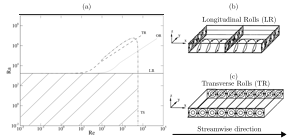
\includegraphics[width=\textwidth]{Background/Figures/RBP/RBP.pdf}
    \caption{(a) Neutral stability curves of longitudinal rolls (LR), oblique rolls (OR), transverse rolls (LR) and Tollmien-Schlicting (TS) waves, adapted from \protect\cite{john_soundar_jerome_transient_2012}. The shaded area refers to damped perturbations. Sketch of (b) longitudinal and (c) transverse rolls, adapted from \protect\cite{kelly_onset_1994}.}
    \label{fig:primary_instabilities}
\end{figure}
This section describes the developments of Rayleigh-B\'{e}nard Poiseuille (RBP) flows, integrating key findings from both plane Poiseuille flow (PPF) and Rayleigh-B\'{e}nard convection (RBC) systems discussed in \S \ref{sec:bkgrd_transitional} and \S \ref{sec:bkgrd_RBC} respectively.
The neutral stability curves in the Rayleigh-B\'{e}nard Poiseuille (RBP) comprising of both plane Poisueuille flow (PPF) and Rayleigh-B\'{e}anrd convection (RBC) systems, are bounded by the onset of Tollmien-Schlicting waves at $Re_{c} = 5772.22$ \citep{orszag_accurate_1971}, and by the onset of convection rolls at $Ra_c = 1708$ \citep{pellew_maintained_1940}, respectively.
% In RBP systems, the imposed mean Poiseuille flow in the RBP system breaks the rotational symmetry of the convection rolls, categorising them based on their orientation to the mean flow direction, namely: longitudinal ($\alpha= 0, \beta \neq 0$), transverse ($\alpha \neq 0, \beta = 0$) and oblique rolls ($\alpha \neq 0, \beta \neq 0$).
In RBP systems, the imposed mean Poiseuille flow in the RBP system breaks the rotational symmetry of the convection rolls, categorising them based on their orientation to the mean flow direction, namely: longitudinal, transverse and oblique rolls.
% Due to the imposed mean flow, the convection rolls are not rotationally invariant, and their orientation with respect to the mean matters.
% Generally, convection rolls that are aligned, diagonal and perpendicular to the mean flow are referred to longitudinal, oblique and transverse rolls.
\textcolor{red}{Primary} instabilities were first investigated by \cite{gage_stability_1968} in an infinitely extended layer.
For longitudinal rolls, the linearised system reduces to the classical RBC problem.
Thus, the critical Rayleigh number remains unchanged at $Ra_{\parallel} = Ra_{c} = 1708.8$ with a critical wavenumber, $\alpha_{\parallel} = \alpha_{c} = 3.13$, independent of \textcolor{red}{the} Reynolds and Prandtl number \citep{pellew_maintained_1940, kelly_onset_1994}.
In contrast, the critical Rayleigh number for the onset of transverse rolls increases with $Re$, and is also dependent on $Pr$ \citep{gage_stability_1968, muller_transversal_1992, nicolas_two-dimensional_1997}.
The critical Rayleigh number for the onset of obliqued rolls can \textcolor{red}{be obtained} by applying a Squire transformation \citep{squire_stability_1933} to transverse roll system.
For a given $Ra$, the corresponding critical $Re$ for the onset of oblique rolls is higher than that for transverse rolls \citep{gage_stability_1968}.
% The critical Rayleigh number for the onset of obliqued rolls are obtained by performing a Squire transformation on the linearised transverse roll system where for a given $Ra$, the critical $Re$ of oblique rolls is higher than the critical $Re$ for transverse rolls \citep{gage_stability_1968}.
The neutral stability curves for the three different rolls are illustrated in figure \ref{fig:primary_instabilities}.
% The neutral stability curves associated with the transverse rolls (TR), oblique rolls (OR) and longitudinal rolls (LR) are shown in figure \ref{fig:primary_instabilities}.

Experimental studies in channels with large transverse aspect ratios (i.e. span-to-depth) showed the onset of longitudinal rolls \citep{akiyama_experiments_1971,ostrach_heat_1975,fukui_longitudinal_1983}, while transverse rolls are more prevalent in narrower channels \citep{luijkx_existence_1981,ouazzani_etude_1989,ouazzani_etude_1990}.
Linear stability analysis of longitudinal rolls for finite channels confirms that $Ra_\parallel$ remains fairly independent for transverse aspect ratios greater than five, and increases quickly below that.
Hence, for small $Re$, critical Rayleigh number of transverse rolls is smaller than that of longitudinal rolls, $Ra_\perp < Ra_\parallel$, giving rise to transverse rolls \citep{nicolas_linear_2000}.
% , $Ra_\perp$,  $Ra_\parallel$ in narrow channels for small Reynolds numbers \citep{nicolas_linear_2000}, providing support for the preference of transverse rolls in narrow channels.
% Indeed, linear stability analysis of narrow channel reveal that the $Ra_{\parallel}$ are increased relative to the $Ra_\perp$ for small $Re$ \citep{nicolas_linear_2000}.
% \st{However, temporal linear stability analysis could not explain the observations by} \cite{ouazzani_etude_1990}\st{, where the laminar Poiseuille flow persisted in the same parameter space where transverse rolls were expected.}
However, laminar Poiseuille flow where observed in the same parameter space where transverse rolls were expected from linear stability analysis \cite{ouazzani_etude_1989}.
% where reported laminar Poiseuille flow in the $Ra, Re$ parameter space where transverse rolls are expected based on temporal linear stability analysis.
% However, linear temporal stability analysis failed to explain the experimental results from \cite{ouazzani_etude_1990}, where a laminar Poiseuille is observed in the parameter space where transverse rolls are expected.
This discrepancy was resolved by \cite{muller_transversal_1992}, who showed that transverse rolls may be convectively or absolutely unstable, with the transition boundary corroborating with experimental data.
Later, \cite{carriere_convective_1999} \textcolor{red}{showed} that longitudinal rolls are always convectively unstable.
% can be either convectively or absolutely unstable, and the boundary between them matches with the experimental results of \cite{ouazzani_etude_1990}.
% By considering the response from three-dimensional impulse, \cite{carriere_convective_1999} further demostrated that the longitudinal rolls, unlike the transverse rolls, are always convectively unstable.
% The critical Rayleigh number for oblique and transverse rolls matches that of RBC at $Re=0$ due to horizontal isotropy, but increases as $Re$ increases, depending on $Pr$, i.e., $Ra_{\perp} = f(Re,Pr)
Nonmodal stability analysis of \textcolor{red}{RBP} by \cite{john_soundar_jerome_transient_2012} \textcolor{red}{showed} that the optimal transient growth is primarily dominanted by streamwise rollers similar to those of PPF \citep{reddy_energy_1993}, with a spanwise wavenumber of $\beta_{opt} \approx 2.05$.
The maximum amplifcation factor, $G_{max}$ increases modestly with $Ra$, and the critical wavenumber approaches $\alpha_{\parallel}$, indicative of longitudinal rolls.
% Nonmodal stability analyses of subcritical RBP indicate that the optimal transient growth $G_{max}$ increases gradually with $Ra$.
% The wavenumber of the optimal initial conditions, $\beta_{max}$, resembles that observed in shear flows \citep{reddy_energy_1993}, and gradually approaches the critical wavenumber of convection rolls, $\alpha_{\parallel}$, as $Ra$ increases \citep{john_soundar_jerome_transient_2012}.
% For $Re > 0$, the longitudinal rolls appear as the dominant primary instability \citep{gage_stability_1968}.
% Since longitudinal rolls are the dominant primary instability for $Re > 0$ in infinite domains, their secondary stability have been analysed by \cite{clever_instabilities_1991}.

For $Re > 0$ in infinite domains, the longitudinal rolls emerge as the dominant primary instability \citep{gage_stability_1968}, and their secondary stability was analysed by \cite{clever_instabilities_1991}.
They identified a time-dependent, wavy instability near $Re \sim 100$, giving rise to tertiary solutions in the form of wavy rolls.
These wavy rolls have been observed experimentally and \textcolor{red}{was} found to be convectively unstable \citep{pabiou_observations_2003, pabiou_wavy_2005, nicolas_characterisation_2010}.
\cite{clever_instabilities_1991} also hypothesised that the wavy rolls are less efficient at transporting heating than longitudinal rolls for the same $Ra$, which was later confirmed numerically by \cite{nicolas_influence_2012}.
The influence of finite transverse aspect ratios on the onset of wavy rolls have also been studied \citep{xin_stability_2006, nicolas_characterisation_2010}, where the critical $Ra$ was found to be approximately 1.5 times higher than in infinite domains \cite{clever_instabilities_1991}.
Furthermore, the effect of external excitation has been explored, showing that increased excitation amplitude can reduce the development length required for the formation of wavy roll \citep{nicolas_characterisation_2010,nicolas_influence_2012}.
In the turbulent regime, shear driven turbulence has been shown to enhance heat transport in RBP flows \citep{scagliarini_heat_2014, scagliarini_law_2015, pirozzoli_mixed_2017}.
% In finite streamwise extensions of RBP flows, the onset of convection rolls and the heat flux variations due to entrance effects have been investigated \citep{mahaney_effect_1988,lee_effect_1991,nonino_laminar_1991}.
Extensions of the RBP configuration, such as flows over wavy walls or with sinusoidal thermal forcing have been investigated, potentially offering a reduction in drag and enhancing heat transport \citep{hossain_drag_2012,hossain_drag_2016,hossain_role_2020}.
% RBP flows with sinusoidal heating and wavy walls have also been studied \citep{hossain_spectral_2021}.
For a comprehensive overview of RBP flows, the reader is referred to the reviews by \cite{kelly_onset_1994} and \cite{nicolas_revue_2002}.

%%%%%%%%%%%%%%%%
% THESIS OUTLINE
%%%%%%%%%%%%%%%%

\section{Thesis Outline}\label{sec:bkgrd_thesis_outline}

% The governing equations of the fluid motion in given by the Navier-Stokes equations with Boussinessq approximations,
% \begin{equation}
%     \frac{\partial \mathbf{u}}{\partial t} + (\mathbf{u} \cdot \nabla) \mathbf{u} = -\frac{1}{\rho} \nabla p + \nu \nabla^2 \mathbf{u} + g\beta(T-T_0).
% \end{equation}`
% \begin{equation}
%     \frac{\partial T}{\partial t} + (\mathbf{u} \cdot \nabla)T = \kappa \nabla^2 T,
% \end{equation}
% \begin{equation}
%     \nabla  \cdot \mathbf{u} = 0.
% \end{equation}
% with arbitrary Dirichlet and Neumann boundary conditions.
% \begin{equation}
%     \mathbf{u}_d, p_d, T_d \in \Omega_d, \quad \nabla\mathbf{u}_N, p_N, T_N \in \partial\Omega_N.
% \end{equation}
% where $\mathbf{u}, T, p$ refers to the velocity, temperature and pressure fields, primitive variables that are not known a priori and $\rho, \nu, \kappa$ refers to the properties of the fluid, namely, density, kinematic viscosity and thermal diffusivity.
% For a given set of fluid properties $\rho, \nu, \kappa$ and geometric properties $L^*, t^*, u^*$ referring to an arbitrary length-, time- and velocity-scale, we are primarily interested in the behaviour of the fluid i.e if its laminar or turbulent.
% In other words, we have a six control parameters that describes a fluid flow of interest.
% To reduce the number of control parameters, we can suitably nondimensionalise the primitive variables by a velocity scale $u_c$, length scale, $L_x$, and time scale $u_c/L_x$, where $u_c$ refers to the centreline velocity of a laminar flow and $L_x$ refers to the streamwise length of the domain.
% The nondimensional equations with Boussienessq approximations are now given as,
% \begin{equation}
%     \frac{\partial \mathbf{u}}{\partial t} + (\mathbf{u}\cdot\nabla)\mathbf{u} = -\nabla p + \frac{1}{Re}\nabla^2 \mathbf{u} + \frac{Ra}{Re^2Pr} \theta
% \end{equation}
% \begin{equation}
%     \frac{\partial \theta}{\partial t} + (\mathbf{u} \cdot \nabla)\theta = \frac{1}{RePr}\nabla^2 \theta,
% \end{equation}
% \begin{equation}
%     \nabla \cdot \mathbf{u} = 0.
% \end{equation}
% where $\mathbf{u}, \theta, p$ refers to the nondimensionalised velocity, temperature and presure.
In this thesis, I \textcolor{red}{will} focus on the transitional behaviour of fluid flow in Rayleigh-B\'{e}nard Poiseuille systems by conducting direct numerical simulations and linear stability analysis.
% addressing questions related to the onset of instabilities due to shear and buoyancy, and the (possible) competitive between shear and buoyancy driven instabilities.
Notably, the onset of instabilities \textcolor{red}{may} give rise to flow regimes that are neither fully laminar nor fully turbulent.
For clarity, we refer to these flow regimes collectively as the transitional regime.
% I would like to preface that while this thesis is dealing with onset of instabilities, it does not clearly indicate that the onset of such instabilities necessarily lead to turbulence, hence, for terminology sake, we shall be looking into transitional regimes where the fluid neither laminar nor turbulent.

While significant progress has been made \textcolor{red}{towards the} understanding \textcolor{red}{of} the transition process of Rayleigh-B\'{e}nard convection and plane Poiseuille flows separately, their combined effects remains largely unexplored.
% There had been significant progress in our understanding of the instabilities of Rayleigh-B\'{e}nard convection and plane Poiseuille flows, their combined effects are not known.
For instance, do convection rolls promote the transition to shear driven turbulence?
And conversely, how does shear affect the bistable \textcolor{red}{system} between ideal straight rolls (ISRs) and spiral defect chaos (SDC)?
These questions are \textcolor{red}{explored} in \S \ref{chap:3}.

Although the co-existence of ISRs and SDC as bistable states in Rayleigh-B\'{e}nard convection is well established, the existence of multiple states raises further questions about the notion of bistability.
In \S \ref{chap:4}, we investigate the state-space structure \textcolor{red}{of} ISRs and SDC, identifying several stable invariant solutions referred to as \textit{elementary} states that underpin the pattern formation of SDC. 
% We explore the state space structure of ideal straight rolls (ISRs) and spiral defect chaos (SDC) in \S \ref{chap:4}, identifying several stable invariant states referred to as \textit{elementary} states, underpinning the pattern formation of SDC.
% Subsequently, we explore the state space structure of the bistable system between ISRs and SDC in \S \ref{chap:4}.
% \begin{enumerate}
% \item From an academia point of view, the 
% Within academia, the onset and transition to turbulence in Rayleigh-B\'{e}nard Poiseuille flows remains poorly understand.
% 
% \end{enumerate}

The thesis is structured \textcolor{red}{as} follows: 
\begin{enumerate}

    \item \S \ref{chap:1} provides the introduction and a review of relevant literature.
    \item \S \ref{chap:2} \textcolor{red}{describes} the numerical methods, \textcolor{red}{such as} the spectral/\textit{hp} element method, algorithms for solving the Navier-Stokes equations, linear stability analysis and edge tracking.
    \item \S \ref{chap:3} introduces the $Ra-Re$ phase space of RBP flows, with a particular focus on the role of longitudinal rolls in sustaining turbulence. We introduce the \textit{thermally-assisted sustaining process} - an alternative route towards turbulence via linearly unstable longitudinal rolls
    \item \S \ref{chap:4} explores the organisation of the state space of spiral defect chaos and ideal straight rolls $Ra = 2903$, accompanied by \textit{elementary} states, edge states and highlight some pathways towards SDC
    \item Finally, \S \ref{chap:5} conludes this thesis and suggests possible avenues of future research.
\end{enumerate}
.

% \begin{enumerate}
%    \item Academic motivation - flow structures, statistics, transition.
%    \item Application motivation - shear, heat transfer. Chip cooling, thin-film fabrication and atmospheric boundary layer.
% \end{enumerate}
% We seek to investigate the influence of unstable stratification quantified by Rayleigh number $Ra$, on the behaviour tuburlent-laminar bands. 
% The onset of convection occurs at a critical Rayleigh number of $Ra_c > 1708$, in the form of a pair of convection rolls.
% When aligned in the streamwise direction, the convection rolls are seemingly analogous to a pair of counter-rotating vortices, an optimal initial condition for transient growth. 
% Our investigation naturally answers a few questions related to turbulent-laminar bands.
% For example, does the onset of turbulent-laminar bands, $Re_{cr}$ decrease with increasing $Ra$?
% Do $Ra$-effects influence the structure of turbulent-laminar bands i.e band angle/width? 
% 
% The answers to our research will have important implications Rayleigh-B\'{e}nard Poiseuille flows, ubiquitous in atmospheric, geophysical and engineering flows.
